% The document class supplies options to control rendering of some standard
% features in the result.  The goal is for uniform style, so some attention 
% to detail is *vital* with all fields.  Each field (i.e., text inside the
% curly braces below, so the MEng text inside {MEng} for instance) should 
% take into account the following:
%
% - author name       should be formatted as "FirstName LastName"
%   (not "Initial LastName" for example),
% - supervisor name   should be formatted as "Title FirstName LastName"
%   (where Title is "Dr." or "Prof." for example),
% - degree programme  should be "BSc", "MEng", "MSci", "MSc" or "PhD",
% - dissertation title should be correctly capitalised (plus you can have
%   an optional sub-title if appropriate, or leave this field blank),
% - dissertation type should be formatted as one of the following:
%   * for the MEng degree programme either "enterprise" or "research" to
%     reflect the stream,
%   * for the MSc  degree programme "$X/Y/Z$" for a project deemed to be
%     X%, Y% and Z% of type I, II and III.
% - year              should be formatted as a 4-digit year of submission
%   (so 2014 rather than the accademic year, say 2013/14 say).


\documentclass[ % the name of the author
                    author={Callum Pearce},
                % the name of the supervisor
                supervisor={Dr. Neill Campbell},
                % the degree programme
                    degree={MEng},
                % the dissertation    title (which cannot be blank)
                     title={How effective are Temporal difference learning methods for reducing the number of zero contribution light paths, while still accurately approximating Global Illumination in Path tracing?},
                % the dissertation subtitle (which can be blank)
                  subtitle={},
                % the dissertation     type
                      type={research},
                % the year of submission
                      year={2019} ]{dissertation}

\begin{document}

% =============================================================================

% This section simply introduces the structural guidelines.  It can clearly
% be deleted (or commented out) if you use the file as a template for your
% own dissertation: everything following it is in the correct order to use 
% as is.

\section*{Prelude}
\thispagestyle{empty}

A typical dissertation will be structured according to (somewhat) standard 
sections, described in what follows.  However, it is hard and perhaps even 
counter-productive to generalise: the goal is {\em not} to be prescriptive, 
but simply to act as a guideline.  In particular, each page count given is
important but {\em not} absolute: their aim is simply to highlight that a 
clear, concise description is better than a rambling alternative that makes
it hard to separate important content and facts from trivia.

You can use this document as a \LaTeX-based~\cite{latexbook1,latexbook2} 
template for your own dissertation by simply deleting extraneous sections
and content; keep in mind that the associated {\tt Makefile} could be of
use, in particular because it automatically executes  to 
deal with the associated bibliography.  

You can, on the other hand, opt {\em not} to use this template; this is a 
perfectly acceptable approach.  Note that a standard cover and declaration 
of authorship may still be produced online via
\[
\mbox{\url{http://www.cs.bris.ac.uk/Teaching/Resources/cover.html}}
\]

% =============================================================================

% This macro creates the standard UoB title page by using information drawn
% from the document class (meaning it is vital you select the correct degree 
% title and so on).

\maketitle

% After the title page (which is a special case in that it is not numbered)
% comes the front matter or preliminaries; this macro signals the start of
% such content, meaning the pages are numbered with Roman numerals.

\frontmatter

% This macro creates the standard UoB declaration; on the printed hard-copy,
% this must be physically signed by the author in the space indicated.

\makedecl

% LaTeX automatically generates a table of contents, plus associated lists 
% of figures, tables and algorithms.  The former is a compulsory part of the
% dissertation, but if you do not require the latter they can be suppressed
% by simply commenting out the associated macro.

\tableofcontents
\listoffigures
\listoftables
\listofalgorithms
\lstlistoflistings

% The following sections are part of the front matter, but are not generated
% automatically by LaTeX; the use of \chapter* means they are not numbered.

% -----------------------------------------------------------------------------

\chapter*{Executive Summary}

\begin{comment}
{\bf A compulsory section, of at most $1$ page} 
\vspace{1cm} 

\noindent
This section should pr\'{e}cis the project context, aims and objectives,
and main contributions (e.g., deliverables) and achievements; the same 
section may be called an abstract elsewhere.  The goal is to ensure the 
reader is clear about what the topic is, what you have done within this 
topic, {\em and} what your view of the outcome is.

The former aspects should be guided by your specification: essentially 
this section is a (very) short version of what is typically the first 
chapter.  Note that for research-type projects, this {\bf must} include 
a clear research hypothesis.  This will obviously differ significantly
for each project, but an example might be as follows:

\begin{quote}
My research hypothesis is that a suitable genetic algorithm will yield
more accurate results (when applied to the standard ACME data set) than 
the algorithm proposed by Jones and Smith, while also executing in less
time.
\end{quote}

\noindent
The latter aspects should (ideally) be presented as a concise, factual 
bullet point list.  Again the points will differ for each project, but 
an might be as follows:

\begin{quote}
\noindent
\begin{itemize}
\item I spent $120$ hours collecting material on and learning about the 
      Java garbage-collection sub-system. 
\item I wrote a total of $5000$ lines of source code, comprising a Linux 
      device driver for a robot (in C) and a GUI (in Java) that is 
      used to control it.
\item I designed a new algorithm for computing the non-linear mapping 
      from A-space to B-space using a genetic algorithm, see page $17$.
\item I implemented a version of the algorithm proposed by Jones and 
      Smith in [6], see page $12$, corrected a mistake in it, and 
      compared the results with several alternatives.
\end{itemize}
\end{quote}
\end{comment}

In the field of Computer Graphics, Path tracing is an algorithm which 
accurately approximates global illumination in order to produce 
photo-realistic images. Path tracing has traditionally been known to 
trade speed for image quality. This is due to the lengthy process of accurately 
finding each pixels colour, whereby many light rays are 
fired through each pixel into scene, then directions for each ray are 
continually sampled until it intersects with a light source. Due to 
this, a variety of Importance sampling algorithms have been designed 
to avoid sampling directions which lead to rays contributing no light 
to the rendered image. The paths formed by sampling rays in these 
directions are known as zero contribution light paths. By not sampling 
zero contribution light paths, it is possible to significantly reduce 
the noise in rendered images using the same number of sampled rays per 
pixel in path tracing\\

Recently a Temporal Difference learning method was used by Nvidia to
achieve impressive results in Importance sampling within a Path tracer.
The algorithm essentially learns which directions light is coming from for
a given point in the scene. It then uses importance sampling to favour shooting
rays stored in those directions, reducing the number of zero contribution light paths
sampled. With this success, there is plenty of potential to experiment with
other Temporal Difference learning methods, particularly Deep Q-Learning.
It is also important to assess both of these methods on their ability to 
accurately approximate Global Illumination to produce photo-realistic images.
From this, my goal is to investigate the ability of two different temporal
difference learning algorithms ability to reduce the number of zero contribution
light paths in path tracing, whilst still accurately approximating global illumination.
More specifically, the first temporal difference learning method will be that proposed
by Nvidia, and the second will be my designed Neural-Q path tracing algorithm.
I will be comparing these two methods in order to test the following hypothesis:

\begin{quote}
The Neural-Q  path tracer is further able to reduce
the number of zero contribution light paths than an Expected SARSA
Path tracer proposed by Nvidia, whilst still accurately simulating Global Illumination.
\end{quote}

\noindent
\textbf{Outcomes}
\begin{itemize}
\item Which is better able to reduce the number of zero contribution light paths expected SARSA or Deep Q-learning
\item Can Expected SARSA learning handle multiple lights well in a scene \& deep q-learning
\end{itemize}

\noindent
\textbf{Main areas of work}
\begin{itemize}
\item I have written $x$ lines of code to build a  Path tracing engine from scratch which supports a variety of GPU accelerated Path tracing algorithms I have experimented with.

\item I have spent $x$ hours researching into the field of efficient light transport simulation for ray-tracing techniques.

\item I have spent $x$ hours researching into Reinforcement learning, particularly Temporal Difference learning and Deep Reinforcement learning, neither of which I have been taught before.

\item I spent $x$ hours implementing and validating the on-line Expected SARSA Path tracing algorithm proposed by Nvidia, which required me to implement the Irradiance Volume data structure as a prerequisite.

\item I have spent $x$ hours designing, implementing and analysing my own on-line Deep Q-learning Path tracing algorithm, along with a neural network architecture
designed for the algorithm.

\end{itemize}


% -----------------------------------------------------------------------------

\chapter*{Supporting Technologies}

\begin{comment}
{\bf A compulsory section, of at most $1$ page}
\vspace{1cm} 

\noindent
This section should present a detailed summary, in bullet point form, 
of any third-party resources (e.g., hardware and software components) 
used during the project.  Use of such resources is always perfectly 
acceptable: the goal of this section is simply to be clear about how
and where they are used, so that a clear assessment of your work can
result.  The content can focus on the project topic itself (rather,
for example, than including ``I used \mbox{\LaTeX} to prepare my 
dissertation''); an example is as follows:

\begin{quote}
\noindent
\begin{itemize}
\item I used the Java {\tt BigInteger} class to support my implementation 
      of RSA.
\item I used a parts of the OpenCV computer vision library to capture 
      images from a camera, and for various standard operations (e.g., 
      threshold, edge detection).
\item I used an FPGA device supplied by the Department, and altered it 
      to support an open-source UART core obtained from 
      \url{http://opencores.org/}.
\item The web-interface component of my system was implemented by 
      extending the open-source WordPress software available from
      \url{http://wordpress.org/}.
\end{itemize}
\end{quote}
\end{comment}


\begin{enumerate}
\item I used the \verb|SDL2|  library for displaying and saving rendered 
images from my Path tracing engine.

\item I used the \verb|OpenGL| mathematics library to support low level 
operations in my Path tracing engine. It includes GPU accelerated 
 implementations for all of its functions.
 
\item I used the \verb|CUDA Toolkit 10.1| parallel computing platform for
 accelerating Path tracing algorithms. This means the \verb|CUDA nvcc|
 compiler must be used to compile my Path tracing engine.

\item All experiments were run on my own desktop machine with an
Nvidia \verb|1070Ti| GPU, Intel \verb|i5-8600K| CPU and $16$GB of RAM.

\item I used the C++ API for the \verb|Dynet| neural network framework 
to implement all of my Neural Network code as it is able to be compiled
by the \verb|CUDA| compiler.
\end{enumerate}

% -----------------------------------------------------------------------------

\chapter*{Notation and Acronyms}

\begin{comment}
{\bf An optional section, of roughly $1$ or $2$ pages}
\vspace{1cm} 

\noindent
Any well written document will introduce notation and acronyms before
their use, {\em even if} they are standard in some way: this ensures 
any reader can understand the resulting self-contained content.  

Said introduction can exist within the dissertation itself, wherever 
that is appropriate.  For an acronym, this is typically achieved at 
the first point of use via ``Advanced Encryption Standard (AES)'' or 
similar, noting the capitalisation of relevant letters.  However, it 
can be useful to include an additional, dedicated list at the start 
of the dissertation; the advantage of doing so is that you cannot 
mistakenly use an acronym before defining it.  A limited example is 
as follows:
\end{comment}

\begin{quote}
\noindent
\begin{tabular}{lcl}
TD learning    &:    & Temporal Difference learning\\
\end{tabular}
\end{quote}

% -----------------------------------------------------------------------------

\chapter*{Acknowledgements}

{\bf An optional section, of at most $1$ page}
\vspace{1cm} 

\noindent
It is common practice (although totally optional) to acknowledge any
third-party advice, contribution or influence you have found useful
during your work.  Examples include support from friends or family, 
the input of your Supervisor and/or Advisor, external organisations 
or persons who  have supplied resources of some kind (e.g., funding, 
advice or time), and so on.

\subsection{Plan}
\begin{enumerate}
\item Carl Henrik Ek - Validating my understanding of deep reinforcement learning
\item Neill Campbell - Deep reinforcement learning strategy
\end{enumerate}

% =============================================================================

% After the front matter comes a number of chapters; under each chapter,
% sections, subsections and even subsubsections are permissible.  The
% pages in this part are numbered with Arabic numerals.  Note that:
%
% - A reference point can be marked using \label{XXX}, and then later
%   referred to via \ref{XXX}; for example Chapter\ref{chap:context}.
% - The chapters are presented here in one file; this can become hard
%   to manage.  An alternative is to save the content in seprate files
%   the use \input{XXX} to import it, which acts like the #include
%   directive in C.

\mainmatter

% -----------------------------------------------------------------------------

\chapter{Contextual Background}
\label{chap:context}

% I don't like this, needs to be more like the opening of a book chapter 

This chapter explains on a high level what path tracing is and how it accurately 
simulates light transport. Then importance sampling ray directions in light
transport simulation is discussed, and how it can potentially reduce the number 
of zero contribution light paths and the associated benefits with this. Temporal 
difference learning as a branch of reinforcement learning is then introduced, 
along with how it can be used in importance sampling ray directions towards 
light sources. With a conceptual overview of theory my work is based on, I take 
a look at recent work which contributes to real-time accurate light transport 
simulation which my work aims to contribute to. Finally, an overview of the 
objectives and significant challenges of my investigation are described.


\section{Path Tracing for Light Transport Simulation}
\label{sec:conceptual_path_trace}
Path Tracing is a Monte Carlo method for rendering photo-realistic images of 3D 
scenes by accurately approximating global illumination \cite{christensen2016path}.
Figure \ref{fig:path_tracing_overview} summarises on a high level how forward Path tracing produces a 
2D image of a 3D scene. For each pixel multiple rays are shot from the camera through the 
pixel and into the scene. Any ray which intersects with an area light terminates, 
otherwise a new direction is sampled for the ray and it is fired again. This process 
is repeated until all rays have intersected with an area light, at which point the pixel 
colour value can  be found by averaging the colour estimate of each ray fired 
through that pixel. Each rays colour estimate is calculated based on the material 
surface properties it intersects with before intersecting with the light and the
intersected area lights properties. The more rays shot through each pixel (also 
known as samples per pixel), the higher the quality of the rendered image 
becomes, but at a higher computational cost.

\begin{figure}[h!]
\begin{center}
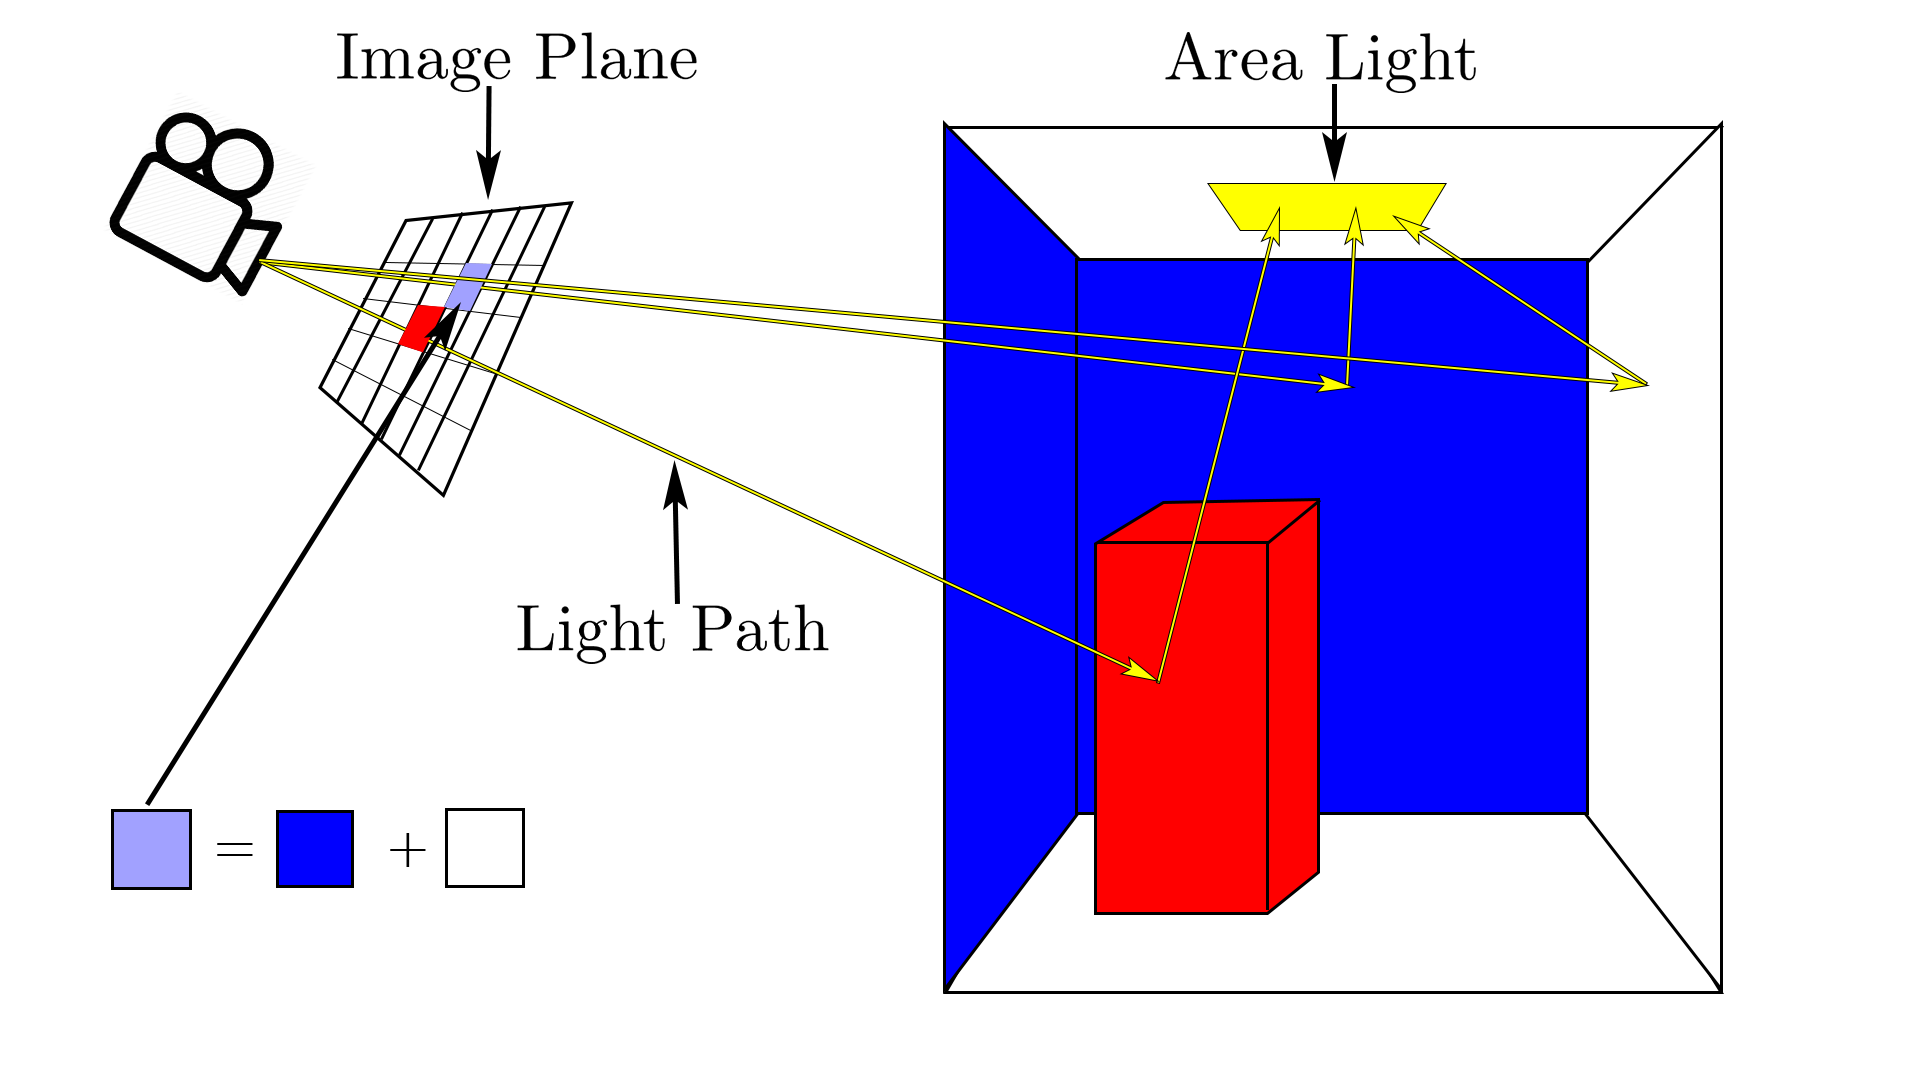
\includegraphics[width=0.8\textwidth]{images/path_tracing.png}    
\end{center}
\caption{An illustration of path tracing, where three light paths are traced from from the camera through a pixel, to the light source in a simple 3D scene.}
\label{fig:path_tracing_overview}
\end{figure}

Path tracing simulates global illumination, meaning it accounts for both direct and 
indirect illumination. Direct illumination being light paths emitted from a light 
source, which reflect off exactly one surface before reaching the camera in the 
scene . Whereas in indirect illumination, light paths reflect 2 or times before
reaching the camera. In Figure \ref{fig:direct_and_global}, an identical scene is shown with only direct illumination
(left) and the other with global illumination (right). The globally illuminated scene displays
a range of effects due to Path tracings ability to accurately simulate light transport, 
which is not the case for the directly illuminated scene. Where light transport simulation
refers to firing and summing up the contributions of light transport paths that connect from the
camera to light sources \cite{keller2016path}, such as those displayed in Figure \ref{fig:direct_and_global}. For 
example, effects such as; (a) colour bleeding which is clear on the white walls by the boxes. (b) Soft shadows of the boxes silhouette. (c) Indirect diffuse lighting
from light transport simulation causes the shadow of the box to not be pitch black.\\

\begin{figure}[h]
\centering
\begin{minipage}{.45\textwidth}
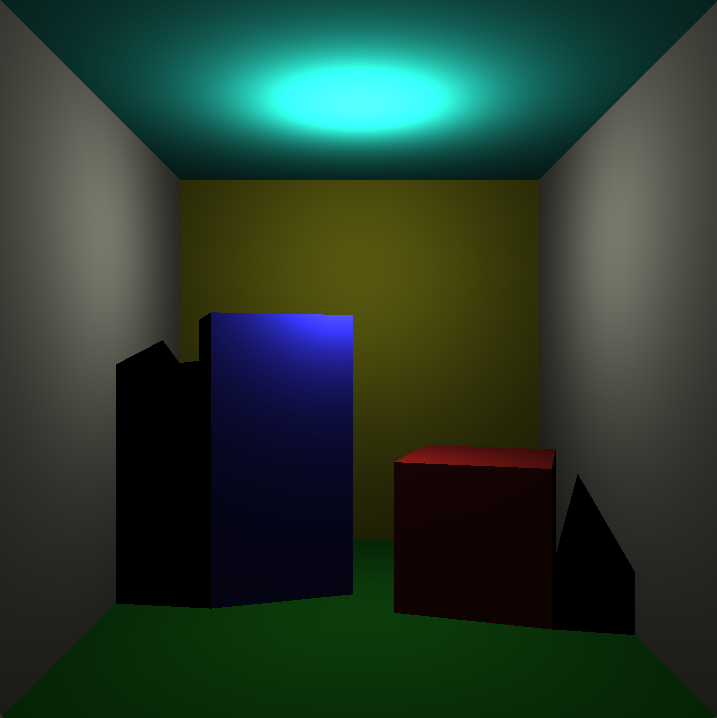
\includegraphics[width=0.99\textwidth]{images/renders/cornell/direct_light.png}    
\subcaption{Direct Illumination}
\end{minipage}\hspace{2em}
\begin{minipage}{.45\textwidth}
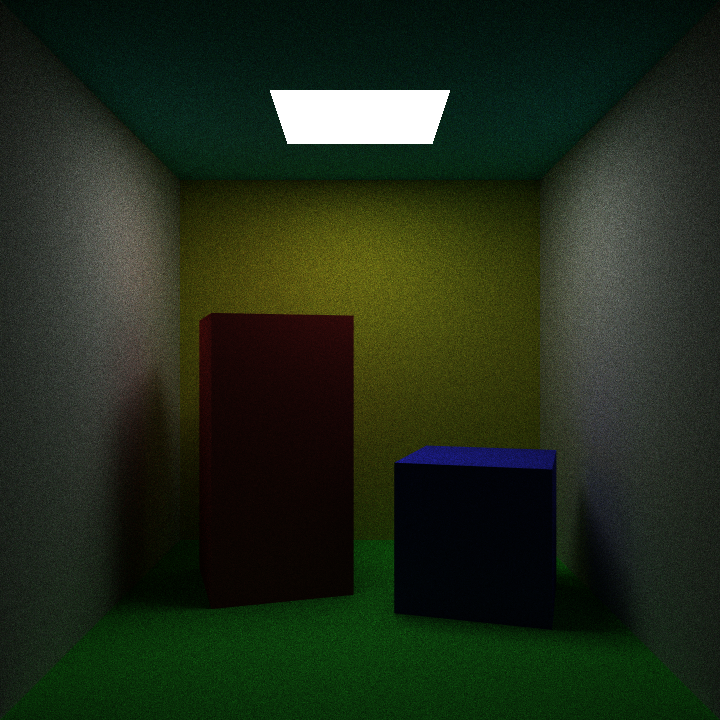
\includegraphics[width=0.99\textwidth]{images/renders/cornell/2048_300_default.png}    
\subcaption{Global Illumination}
\end{minipage}
\caption{Two renders of the Cornell Box, where the left is directly illuminated and the right is globally illuminated.}
\label{fig:direct_and_global}
\end{figure}

Light transport simulation methods are able to produce 
many complex light transport effects by a simple single pass of a rendering algorithm.
This allows artists to increase productivity and perform less manual image tweaking
in the production of photo-realistic images. Due to this, the Computer Graphics 
industry has seen a large resurgence in research and usage of light transport simulation 
rendering methods in the past decade \cite{krivanek2014recent}. \\

My work in this thesis focuses on developing and assessing importance sampling 
techniques using Temporal Difference learning methods for light transport simulation 
in forward Path tracing. In particular, More specifically,
for any intersection point in a 3D scene, I attempt to create an AI agent that learns 
and samples in  directions light is coming from, reducing the total number of 
zero contribution light paths. A zero contribution light path is one whose 
estimated colour values are almost zero for all $(R,G,B)$ components, hence,
they contribute almost no visible difference to the rendered image. We should 
instead focus our sampling on light paths which do contribute to the image,
reducing the noise in pixel values and bringing them closer to their true 
values for the same number of sampled rays per pixel. Meaning, Importance 
sampling can reduce the number of rays needed to be sampled per pixel in 
order to receive a photo-realistic (also known as converged) image from Path 
tracing. An example of this reduction in noise can be see in \ref{fig:noise_reduction_simple_room}, where the 
default forward path tracers output is compared to Nvidia's on-line
reinforcement learning Path tracer which uses Importance sampling. Note, any 
light transport simulation algorithm \cite{jensen1996global, keller2016path} can benefit from the Temporal DIfference learning
schemes which will be described, 
as they are all derived from what is known as the rendering equation. This equation
is used as a mathematical basis of modelling light transport.\\

\begin{figure}[h]
\centering
\begin{minipage}{.45\textwidth}
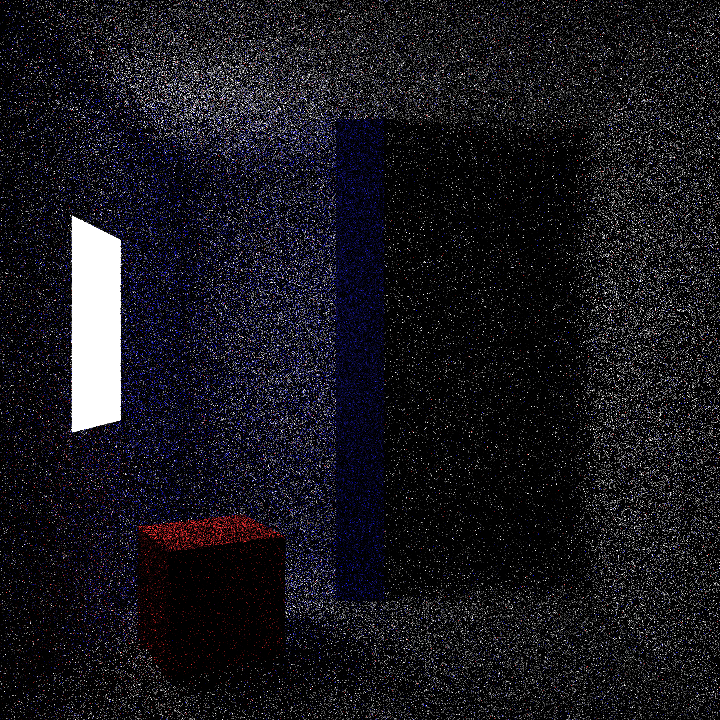
\includegraphics[width=0.99\textwidth]{images/renders/simple_room/default_16.png}    
\subcaption{Default Forward Path Tracer}
\end{minipage}\hspace{2em}
\begin{minipage}{.45\textwidth}
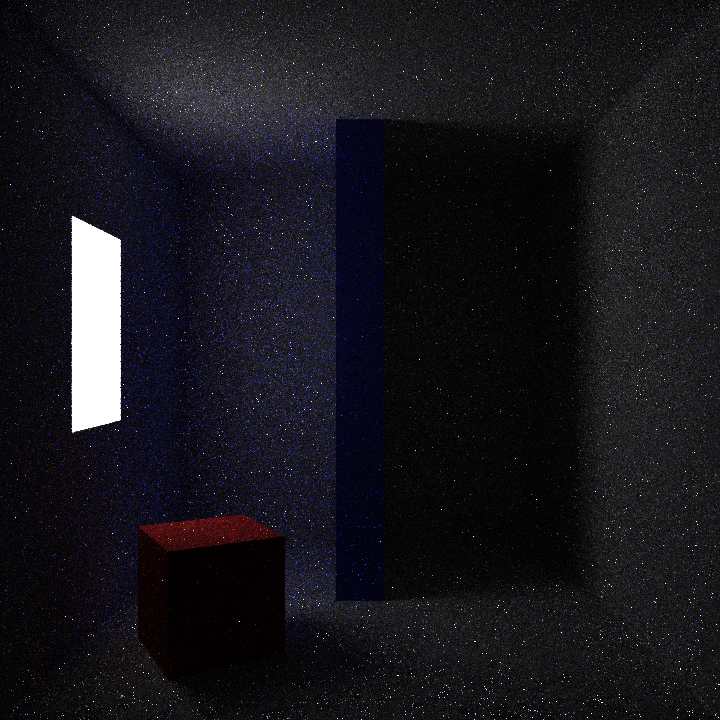
\includegraphics[width=0.99\textwidth]{images/renders/simple_room/reinforcement_16.png}    
\subcaption{Expected Sarsa Path Tracer}
\end{minipage}
\caption{Two renders of a simple room using 16 sampled light paths per pixel. Where one does not use importance sampling in the construction of light paths (left), and the other does so based on a reinforcement learning rule (right). A clear reduction in image noise can be seen.}
\label{fig:noise_reduction_simple_room}
\end{figure}

It is paramount that Importance sampling Path tracing algorithms continue to accurately
simulates global illumination in order to produce photo-realistic images in a single
rendering pass, as this is the major selling point of Path tracing over other 
methods. Therefore, I will also be assessing the accuracy of the global
illumination approximation made by the Importance sampling algorithms compared
to that of the naive forward Path tracing algorithm.

\section{Temporal Difference Learning for Importance Sampling Ray Directions}
\label{sec:td_learn_for_importance}

There are three important unanswered questions up to this point; a) what is temporal
difference learning?  b) How can temporal difference learning methods be 
used to importance sample new ray directions for a given intersection point in 
the scene? c) Why use temporal difference learning methods over other Importance 
sampling methods to do so? 

\subsection{What is Temporal Difference learning?}
Temporal difference learning, which I will refer to from 
here on as TD-learning, are a set of model free Reinforcement learning methods. 
Firstly, Reinforcement learning is the process of an AI agent learning what is the 
best action to take in any given state of the system it exists within, in order to 
maximise a numerical reward signal \cite{sutton2011reinforcement}.
The AI agent is not told which actions are  best to take in a given state, but
 instead it must learn which ones are by trialling them and observing the reward 
signal. Actions taken may not only affect the immediate 
reward, but all subsequent rewards received for taking future actions. For 
example, picture a robot rover whose duty it is to explore the surrounding area 
as much possible. A state in this case is a position in the world it is exploring, 
and its action are the directions to move in for a given distance. If it discovers 
a new area, it receives a positive reward signal. Now, if the robot chooses to 
explore a given area it may not be able to get back from, say a canyon, the 
robot is limited to searching areas reachable from the canyon. Hence, all 
subsequent reward signals are limited to what can be received from exploration 
of the canyon, compared to not entering the canyon and exploring areas which 
can be returned from first.

\begin{comment} %Might need to remove all
As mentioned TD learning methods are model free methods, meaning the methods 
do not require a model of the system dynamics they are placed in, instead they
 learn over time by interacting with the system. In other words, they learn from 
 raw experience  \cite{sutton2011reinforcement}. TD methods update their current
estimates based on a combination of data received from interacting with the 
environment, and partly on their current learned estimates without waiting for the 
final outcome of events, this is known as bootstrapping. To illustrate the concept 
of bootstrapping, imagine you are driving home from work and you wish to estimate 
how long it will take you get home. By following a TD learning method, if you hit 
traffic you can update your current estimate of the time it takes you to drive home
based on this new data, and your pre-existing estimate. Whereas compared to 
another set of Reinforcement learning methods known as Monte Carlo methods, 
you would have to wait until you got home to update your current estimate of how 
long it takes to get home from work. Meaning you have to wait for the final outcome
before learning can begin, which is not the case for TD learning.
\end{comment}

\subsection{Temporal Difference learning methods for Efficient Light Transport Simulation}

One of my main aims to reduce the number of zero contribution light paths sampled 
in Path tracing by the use of TD learning methods. In order to do so I must formulate 
the problem a reinforcement learning problem, which is done in detail in Chapter
\ref{chap:technical}. However for a conceptual overview it suffices to explain what a 
state, action, and reward signal will be in the case of light transport simulation within 
Path tracing:

\begin{itemize}

\item \textbf{State}: A 3D intersection position in the scene for a given ray to sample 
the rays next direction from. 

\item \textbf{Action}: Firing the ray in a given direction (3D vector) from the current 
state.

\item \textbf{Reward Signal}: The amount of light incident from the direction the ray 
was sampled in.

\end{itemize}

In this reinforcement learning setting, we can use TD-learning methods to create 
an AI agent which learns by taking different actions in different states and observes 
their reward signals to find out for each state which actions have the highest valuations.
By then converting the action space into a probability distribution weighted by each
actions learned valuation, the AI agent will more likely sample non-zero contribution 
light paths, reducing noise in rendered images. Note, the term valuation means the 
total expected reward for taking a given action, meaning valuation not only accounts 
for the immediate reward, but the expected reward for taking all future actions to come 
until the ray intersects with a light. Also, for the proposed AI agent, current actions 
can affect future rewards, as when the ray intersects a surface it looses some energy. 
Therefore, future rewards received after many intersections will be discounted 
compared to the reward of received immediately to match this behaviour. This means 
the agent will aim to minimise the average number of intersection a ray makes before 
intersecting with a light source, making it a good metric to test evaluate against to 
determine how well the AI agent is performing.

\subsection{Why use Temporal Difference Learning for Importance Sampling?}

Traditional Importance sampling techniques for path tracing do not take into account 
the visibility of the object from light source. A light blocker is shown in \ref{fig:blocker}, where the 
blocking object stops rays from directly reaching the light. Due to the unknown 
presence of blockers, traditional importance sampling methods can fail to avoid 
sampling zero contribution light paths. Therefore, scenes which are significantly 
affected by blockers will not receive the benefits from traditional Importance sampling 
and can even benefit more from an uniform sampling scheme 
\cite{ramamoorthi2012theory}.\\

\begin{figure}[h!]
\begin{center}
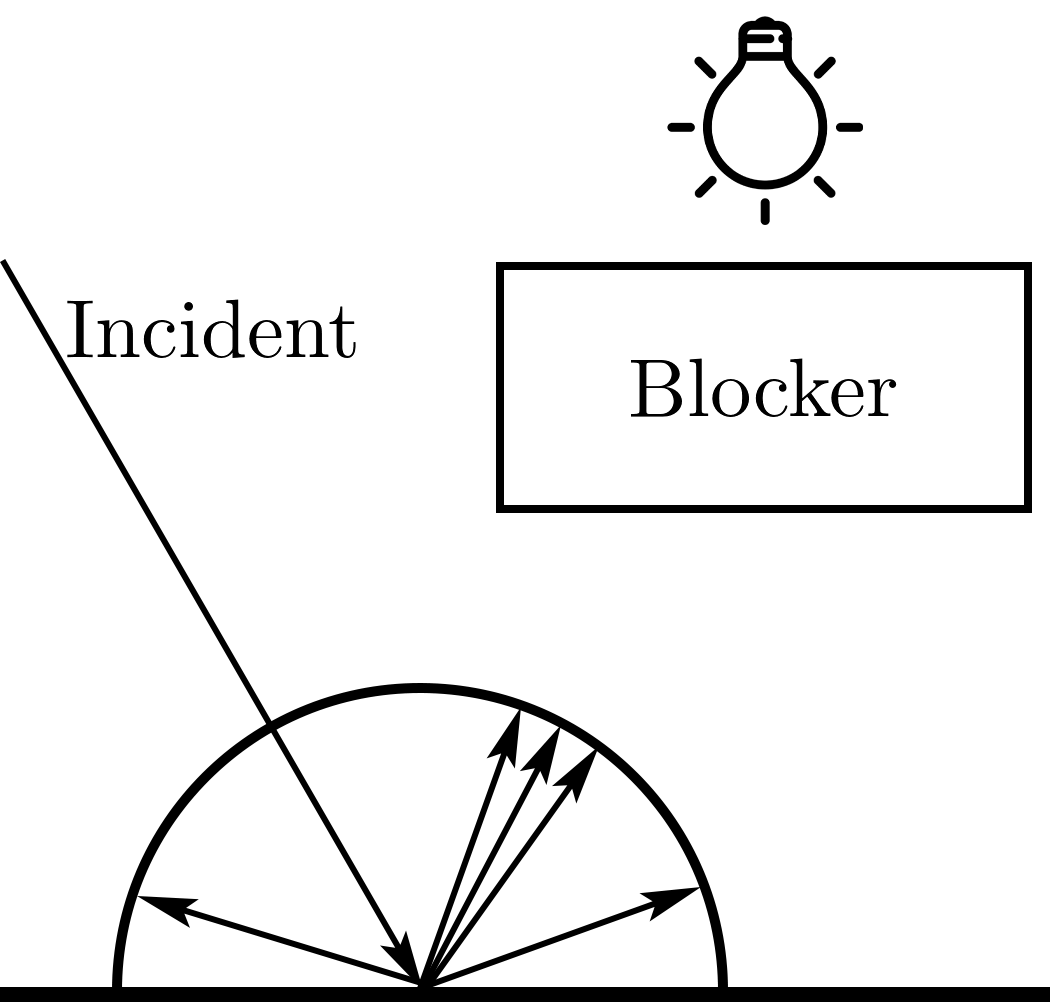
\includegraphics[width=0.3\textwidth]{images/light_blocker.png}    
\end{center}
\caption{An illustration of a light blocker for an importance sampling scheme which does not consider visibility. Each arrow represents a possible direction the light path will be reflected in. Clearly the reflected light path is likely to hit the blocker increasing the likelihood of it becoming a zero-contribution light path.}
\label{fig:blocker}
\end{figure}

Temporal difference learning methods are better equipped to tackle this problem 
\cite{dahm2017learning}. As the AI agent described in the previous section learns 
which directions light is coming from in the scene and concentrates its sampling 
towards these directions. Directions leading to blockers will have a low value, 
hence it is unlikely the AI agent will sample rays in these directions.\\

\section{Motivation}
\label{sec:motivation}

Rendering time of my graphics engine is not something I have tried to heavily 
optimise. I instead focus on producing higher quality images using the same 
number of samples per pixel in light transport simulation in hope that future 
work will find ways of optimising my methods for speed. Therefore, my work 
still aims to contribute to the wider goal seen in computer graphics to use 
accurate light transport simulation in the rendering of photo-realistic images 
for complex scenes in real-time.  Speeding up the methods I use is a large 
topic in itself, requiring a deep investigation into the best software, hardware, 
and parallel programming paradigms to use.\\

\subsection{Real time Rendering using Accurate Light Transport Simulation}
The motivation for using accurate light transport simulation in real-time 
comes from the clear superior visual quality of images rendered using this 
techniques, compared to that of scanline methods which are currently used. 
Where scanline rendering, also known as rasterizing, is the current computer 
graphics industry standard method for real-time rendering. Not only are 
renders for a wide range of scenes clearly superior from methods which 
accurately simulate light transport, but they also scale far better with the 
number of polygons used to build the scenes surfaces. Therefore, scanline 
rendering for scenes with extremely complex geometry in real-time is currently 
not and option. Accurate light transport simulation methods therefore have 
great potential to be used in ultra realistic simulations for applications such 
as scenario planning and virtual reality learning environments \cite{pan2006virtual}. 
Also, many games sell realism as one of their most important features, therefore 
developing photo-realistic graphics in real-time has clear economic incentive for 
the video games industry which was valued at over \$$136$ by the end of 2018 
\cite{bloomberg.com}. An economic incentive can also be seen for the film
industry, where reductions in render times lead to a direct saving on compute 
time, as well as the hardware required to render full length films.

\subsection{Recent Developments}
Due to the incentives, a large amount of research and investment has been focused 
on purpose built hardware and Deep learning  post-processing methods in an 
attempt to bring accurate light transport simulation into real-time. NVIDIA's 
Turing Ray Tracing Technology \cite{nvidia_turing_architecture_whitepaper_2018} 
represents a significant leap in the hardware to support light transport simulation. 
It allows for real-time graphics engines to be a hybrid of both scanline rendering, 
and ray-tracing. The 20 series Turing GPU architecture has significantly improved 
the speed of ray-casting for light transport simulation, and has the capacity for  
simulating 10 Giga Rays per second. However, using this hardware alone with 
current rendering methods is not enough to perform accurate light transport 
simulation for complex scenes in real-time.\\

Post-processing methods are designed to take a noisy input image produced by a 
render which simulates light transport, and then reconstruct the image to remove 
the noise present in the image. Generally these methods rely on pre-trained deep 
neural networks to reconstruct the image far quicker then it would take for the 
renderer to produce an image of the same visual quality \cite{bako2017kernel}. 
Once again NVIDIA has made significant advancements in this area with NVIDIA 
OptiX AI Accelerated Denoiser, which is based on their newly designed recurrent 
denoising autoencoder \cite{chaitanya2017interactive}. OptiX has been successfully 
integrated in to many of the top rendering engines which accurately simulate light
transport, such as RenderMan \cite{christensen2018renderman} and Arnold 
\cite{georgiev2018arnold}. Whilst post-processing has significantly reduced the 
number of samples required to render photo-realistic images, there is still more 
work to be done to produce these images in real-time.\\

By using importance sampling by TD learning to reduce the number of samples 
required for accurate light transport simulation, the same standard of noisy 
image can be fed into an AI accelerated denoiser with fewer samples per pixel 
in light transport simulation. Running a rendering engine optimised in this way on 
purpose built hardware could make accurate light transport simulation for 
rendering photo-realistic images closer than it ever has been to real-time.

\section{Challenges and Objectives}

% Needs work

As previously mentioned, there already exists an example of TD learning used 
for importance sampling ray directions in a forward Path tracer \cite{dahm2017learning}. 
However, further methods of analysis need to be conducted upon this new 
method to determine its performance for reducing the number of zero contribution l
ight paths for different scenes with different settings. It is difficult to assess this as 
there are infinitely many scenes the method can be used to render, so coming to a 
clear conclusion is difficult. Another difficult task is that of designing an algorithm 
for an AI agent to learn what are the favourable directions to sample in a scene are 
using the deep Q-learning method. This includes some important unanswered 
questions, such as; is it possible for a deep neural network to model all Q values for 
a continuous scene space? If so, what is a suitable network architecture? All of 
which I will describe in more depth in Chapter \ref{chap:deep-q}. Then the actual 
task of implementing such an algorithm in a graphics engine written from scratch 
is non-trivial due to the technologies which will need to be combined together. 
The algorithm must also run fast enough to collect large amounts of data from, 
otherwise a justified conclusion on its performance cannot be made. Therefore, 
the algorithm will have to be parallelized and run on a GPU.\\

As previously mentioned, my main goal is to investigate the ability of two 
different temporal difference learning algorithms ability to reduce the number 
of zero contribution light paths in path tracing, whilst still accurately 
approximating global illumination. Which can be broken down in to the 
following objectives:

\begin{enumerate}
\item Reimplement Nvidia's state of the art on-line Temporal 
Difference learning Path Tracer in order to further investigate its ability
to reduce the number of zero contribution light paths.

\item Design and implement an on-line Deep Q-Learning variant of the
Path tracing algorithm and investigate its ability to reduce the number of zero contribution light paths sampled.

\item Assess both Nvidia's state of the art on-line Temporal Difference 
learning Path tracer, and the Deep Q-Learning Path tracer' on their ability 
to accurately simulate Global Illumination.

\end{enumerate}


\begin{comment}
{\bf A compulsory chapter,     of roughly $5$ pages}
\vspace{1cm} 

\noindent
This chapter should describe the project context, and motivate each of
the proposed aims and objectives.  Ideally, it is written at a fairly 
high-level, and easily understood by a reader who is technically 
competent but not an expert in the topic itself.

In short, the goal is to answer three questions for the reader.  First, 
what is the project topic, or problem being investigated?  Second, why 
is the topic important, or rather why should the reader care about it?  
For example, why there is a need for this project (e.g., lack of similar 
software or deficiency in existing software), who will benefit from the 
project and in what way (e.g., end-users, or software developers) what 
work does the project build on and why is the selected approach either
important and/or interesting (e.g., fills a gap in literature, applies
results from another field to a new problem).  Finally, what are the 
central challenges involved and why are they significant? 
 
The chapter should conclude with a concise bullet point list that 
summarises the aims and objectives.  For example:

\begin{quote}
\noindent
The high-level objective of this project is to reduce the performance 
gap between hardware and software implementations of modular arithmetic.  
More specifically, the concrete aims are:

\begin{enumerate}
\item Research and survey literature on public-key cryptography and
      identify the state of the art in exponentiation algorithms.
\item Improve the state of the art algorithm so that it can be used
      in an effective and flexible way on constrained devices.
\item Implement a framework for describing exponentiation algorithms
      and populate it with suitable examples from the literature on 
      an ARM7 platform.
\item Use the framework to perform a study of algorithm performance
      in terms of time and space, and show the proposed improvements
      are worthwhile.
\end{enumerate}
\end{quote}


\textbf{Preliminary}
\begin{enumerate}
\item Path-tracing in industry/ray-tracing in general, why is it important 
and how is the current field moving. Why should we optimise it algorithmically. 
Why should the reader care about path-tracing? - Usage in films, increasing
 interest for real-time simulations and gaming industry which is worth lots of money

\item High level overview of path-tracing: specifically must explain why it takes 
so long and why we care about the number of samples

\item In the path-tracing algorithm, a single pixel's colour is determined by firing 
multiple rays from the camera, through that pixel into the scene and building a 
colour value estimate for each one, then averaging their values to get the pixels 
colour. Each rays colour estimate is computed by estimating a solution to the recursive
Rendering Equation (cite). The path-tracing algorithms estimate to this solution involves 
scattering the ray around the scene until it intersects with a light source. Therefore, if a
 ray is scattered in a direction with zero-light contribution, but other sampled rays are not,
  a noisy estimate is achieved for the pixel value unless many rays are sampled to 
  reduce the effect of this noise. Therefore, avoiding  scattering rays in directions of 
  zero-light power contribution can reduce the number of samples needed to achieve 
  an accurate estimate of a pixels colour value.

\item Work was primarily motivated by Ken \& Dahms paper for modelling the irradiance
 distribution in order to reduce the number of zero-contribution light transport paths 
 traced. Nvidia are world leaders in GPU manufacturing and drive the computer 
 graphics forward.

\item Literature around efficiently simulating light transport - it's applicability to all 
modern used off-line rendering techniques

\item Aims \& Challenges:

\begin{enumerate}
\item Implementing a path-tracer for diffuse surfaces from scratch using only maths 
and pixel libraries as helper functions which can handle imports of a custom scene
\item Accelerating path-tracer on Cuda to get results in a reasonable time
\item Implementing the irradiance volume data-structure and sampling technique which 
can adapt to any size scene
\item Implementing Ken Dahms proposed path-tracing algorithm with nearest neighbour
 search of KD-Tree on a GPU efficiently 
\item Researching reinforcement learning: TD-Learning \& deep reinforcement learning - 
never been taught before, so self taught with resources on-line
\item Training a network on pre-computed Q values to check if it is possible for a neural
 network to learn the irradiance distribution function for a set of points in a scene
\item Designing an algorithm to integrate deep reinforcement learning into the 
rendering pipeline for a path-tracer
\item Choosing a set of metrics to evaluate the algorithms performances on
\item Accelerating the algorithms via Cuda to run on Nvidia GPU
\end{enumerate}

\end{enumerate}
\end{comment}

% -----------------------------------------------------------------------------

\chapter{Technical Background}
\label{chap:technical}

The goal of this section is to give you as the reader a deep understanding of the technical concepts which build on top of one another to reduce the number of zero contribution light paths in path tracing, whilst still accurately approximating global illumination. Initially I introduce Monte Carlo integration to approximate and integral, as well as importance sampling and how it reduces variance in the approximation. Monte Carlo integration is the fundamental method which path tracing relies on, I describe this in detail within the section on Monte Carlo path tracing and physical laws path tracing relies on. With the method of path tracing for rendering images clear, I move on to an introduction on reinforcement learning, as this is what I will be using for importance sampling in path tracing. Here the important concept of a learning the optimal value function is introduced and methods in doing so. In the next section a temporal difference learning rule is applied to the context of light transport simulation. Finally, the Expected Sarsa path tracer introduced by Nvidia \cite{dahm2017learning} is presented, tying in all what has been learnt so far for reducing the number of zero-contribution light paths in path tracing. 

\begin{comment}
Up to this point, I have discussed  what path tracing is and how it approximates global illumination via light transport simulation. As well as, how importance sampling using TD-learning can improve the efficiency of this approximation by avoiding zero contribution light paths. However all descriptions have been at a high a level to make my motivation clear. In this section I describe in detail the rendering equation which path tracing and other Monte Carlo rendering algorithms are based on. I then present the Markov Decision Process and how TD-learning uses this to solve a general class of problems. The derivation of how the rendering equation can be linked to a TD-learning rule is then given, showing how TD-learning is used for importance sampling ray directions in light transport simulation. Finally, the details of my implementation of the expected SARSA path tracer introduced by NVIDIA \cite{dahm2017learning} in 2017 are given.
\end{comment}

\section{Monte Carlo Integration and Importance Sampling}
\label{sec:monte_carlo}
The theory of Monte Carlo integration and importance sampling underpins how the noise in images rendered by path tracing can be reduced when using the same number of sampled rays per pixel. Therefore, it is necessary to have a good understanding of Monte Carlo integration and its properties, as well as importance sampling before applying it to path tracing.

\subsection{Monte Carlo Integration}
\label{sec:monte_carlo_approx}
 Monte Carlo Integration is a technique to estimate the value of an integral, Equation \ref{eq:integral} represents this integral for a one-dimensional function $f$.

\begin{equation}
\label{eq:integral}
F = \int_a^b f(x) dx
\end{equation}

The idea behind Monte Carlo integration is to approximate the integral by uniformly sampling points ($x_i$) to evaluate the integral at, and then averaging the solution to the integral for all the sampled points. More formally, basic Monte Carlo integration approximates a solution to this integral using the numerical solution in Equation \ref{eq:monte_carlo}. Where $\langle F^N \rangle$ is the approximation of $F$ using $N$ samples.

\begin{equation}
\label{eq:monte_carlo}
\langle F^N \rangle = (b - a) \frac{1}{N} \sum^{N-1}_{i=0} f(x_i)
\end{equation}

\begin{equation}
\label{eq:generalized_mc}
\langle F^N \rangle = \frac{1}{N} \sum^{N-1}_{i=0} \frac{f(x_i)}{\frac{1}{(b-a)}} 
 = \frac{1}{N} \sum^{N-1}_{i=0} \frac{f(x_i)}{pdf(x_i)}
\end{equation}

An important property of Monte Carlo Integration is that it produces an unbiased estimate of an integral, meaning average of $\langle F^N \rangle$ is exactly the true value of the integral,$F$ for any $N$ \cite{morokoff1995quasi}. This is presented in Equation \ref{eq:unbiased}, where $p_i$ is the probability of a given of a given approximation $\langle F^N \rangle$. Basic Monte Carlo integration only produces a non-bias estimate when sample points $x_i$ are randomly sampled from a uniform distribution. To extend this to Generalized Monte Carlo integration where sample points may be sampled from any distribution, the function evaluated at point $x_i$ must be divided by the probability density function ($pdf$) evaluated at $x_i$. This is known as generalized Monte Carlo integration and is shown in Equation \ref{eq:generalized_mc}, which from here onwards I will refer to as Monte Carlo integration. Dividing by the $pdf$ ensures the estimate $\langle F^N \rangle$ is unbiased, as areas with a high $pdf$ will be sampled far more, but their contribution weighting ($\frac{1}{pdf}$) to final estimate will be lower. Whereas areas with a low $pdf$ will be sampled less, but their contribution weighting to the final estimate will be higher to offset this.

\begin{equation}
\label{eq:unbiased}
\mathbf{E}[\langle F^N \rangle] = \sum_{i = 0}^{k-1} \langle F^N \rangle_i * p_i =  F
\end{equation}

Another important property of Monte Carlo integration is that by the law of large numbers, as the number of samples ($N$) approaches infinity, the probability of the Monte Carlo approximation ($\langle F^N \rangle$) being equal to the true value of the integral ($F$) converges to $1$. This law is stated in Equation \ref{eq:law_large_numbers}. By this property Monte Carlo Integration works well for multidimensional functions, as convergence rate of the approximation is independent of the number of dimensions, it is just based on the number of samples using in the approximation. Whereas this is not the case for deterministic approximation methods, meaning they  suffer from what is known as the curse of dimensionality. For path tracing, the integral which is approximated is a 2 dimensional function, hence Monte Carlo integration is used. 

\begin{equation}
\label{eq:law_large_numbers}
Pr( \lim_{N \rightarrow \infty} \langle F^N \rangle = F ) = 1
\end{equation}

The standard error of the Monte Carlo integration approximation decreases according to Equation \ref{eq:mc_error}. Where the standard error describes the statistical accuracy of the Monte Carlo approximation. Where $\sigma_N^2$ is the variance of the solutions for the samples  taken, and is calculated by Equation \ref{eq:sample_variance} using the mean of the solutions for the samples taken ($\mu$). Due to Equation \ref{eq:mc_error}, in practice four times as many samples are required to reduce the error of the Monte Carlo integration approximation by a half. Also, the square root of the variance  is equal to the error of the approximation, so from here on when I refer to reducing the variance I am also implying a reduction in the error of the approximation.

\begin{equation}
\label{eq:sample_variance}
\sigma_N^2 = Var(f) = \frac{1}{N-1} \sum_{i=0}^N (f(x_i) - \mu)^2
\end{equation}

\begin{equation}
\label{eq:mc_error}
\text{Standard Error} = \sqrt{Var(\langle F^N \rangle)} = \sqrt{\frac{\sigma_N^2}{N}} = \frac{\sigma_N}{\sqrt{N}}
\end{equation}

\subsection{Importance Sampling for Reducing Approximation Variance}
\label{sec:importance_smapling}

Currently I have only discussed Monte Carlo integration by sampling points $x_i$ to solve the integral using a uniform distribution. However the purpose of introducing Equation \ref{eq:generalized_mc} was to create a custom $pdf$ which can be used for importance sampling to reduce the variance of the Monte Carlo integration approximation. To understand how and why importance sampling works, first observe Figure \ref{fig:constant_function} where a constant function is given with a single sample point evaluated for $f(x)$. This single sample is enough to find the true value for the area beneath the curve i.e. integrate the function with respect to $x$. This is shown in Equation \ref{eq:constant_monte_carlo}, where $p = f(x)$ $ \forall x \in \mathbb{R}$.

\begin{equation}
\label{eq:constant_monte_carlo}
\langle F^N \rangle = (b - a) \frac{1}{N} \sum^{N-1}_{i=0} f(x_i) = (b - a)  \frac{1}{N} \sum^{N-1}_{i=0} p = pb - pa
\end{equation}

However, Figure \ref{fig:non_lin_function} requires many samples to accurately approximate the integral when sampling from a uniform distribution. This is due to the functions complex shape, meaning many samples are required to calculate the are beneath the curve within the Monte Carlo integral approximation. Generally, it requires fewer samples to approximate a function which is closer to being constant function \cite{morokoff1995quasi}.

\begin{figure}[h]
\captionsetup{justification=centering}
\centering
\begin{minipage}{.33\textwidth}
    \hspace*{\fill}%
      \begin{tikzpicture}
	    \begin{axis}[
		    axis lines = left,
		    tick style={draw=none},
		    xticklabels={},
		    yticklabels={},
		    xlabel = $x$,
		    ylabel = {$f(x)$},
		]
		%Below the red parabola is defined
		\addplot [
		    color=red,
		]
		{0.1};
		\addplot[mark=*] coordinates {(0,0.1)} node[]{} ;
		
		\end{axis}
	\end{tikzpicture}
     \caption{Constant Function\\ with a sample point}
  \label{fig:constant_function}
\end{minipage}
\hspace{8em}
\begin{minipage}{.33\textwidth}
    
  \hspace*{\fill}%

    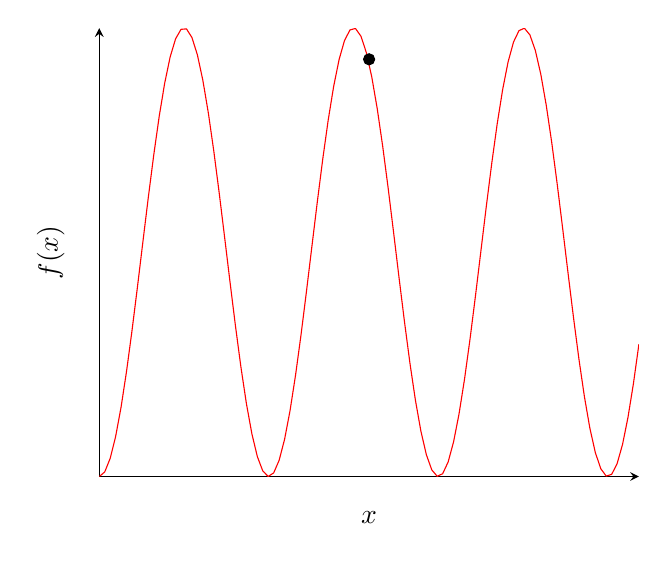
\begin{tikzpicture}
	\begin{axis}[
	    axis lines = left,
	    tick style={draw=none},
	    xticklabels={},
	    yticklabels={},
	    xlabel = $x$,
	    ylabel = {$f(x)$},
	]
	%Below the red parabola is defined
	\addplot [
	    color=red,
	    samples=100,
	]
	{sin(deg(x+5))^2};
    \addplot[mark=*] coordinates {(0,0.93)} node[]{} ;
	\end{axis}
	\end{tikzpicture}  
  \caption{ Non-linear Function\\ with a sample point}
  \label{fig:non_lin_function}
\end{minipage}
\end{figure}

Most functions are not constant, however it is possible to turn any function into one, and this is exactly what can be done within Monte Carlo integration. To convert a function $f$ to a constant function, a function $f'$ can be introduced which produces the same output as $f$ for every input, but scaled by a constant $c$ \cite{scratchapixel_2015}. The function $f$ is then divided by $f'$ to produce a constant function, as shown in Equation \ref{eq:constant_conversion}.

\begin{equation}
\label{eq:constant_conversion}
\frac{f(x)}{f'(x)} = \frac{1}{c}
\end{equation}

This can be applied to Monte Carlo integration stated in Equation \ref{eq:generalized_mc}, by choosing a probability density function ($pdf$) which produces the same output as $f$ for all inputs, but divided by some normlazing constant factor $c$, keeping $pdf$ as a probability distribution. Therefore, we are able to calculate the true value of the integral through Monte Carlo integration as shown in Equation \ref{eq:solve_mc_integration}. Where it turns out $\frac{1}{c}$ is true value for the integral in Equation \ref{eq:integral}.

\begin{equation}
\label{eq:solve_mc_integration}
\langle F^N \rangle = \frac{1}{N} \sum^{N-1}_{i=0} \frac{f(x)}{pdf(x)} = \frac{1}{N} \sum^{N-1}_{i=0} \frac{f(x)}{cf(x)} =  \frac{1}{N} \sum^{N-1}_{i=0} \frac{1}{c} = \frac{1}{c}
\end{equation}

For most cases it is not possible to know the correct probability density function which can convert the Monte Carlo integration problem into integrating a constant function. However, if one has prior knowledge regarding 'important' regions of the functions input space, it is possible to create a probability density function whose shape matches $f$ more closely then a uniform probability distribution. By Important areas of the function input space, I mean areas of the input space which produce a large contribution to the integral of the function. For example in Figure \ref{fig:improtance_correct}, the most important regions are around the top of the functions peak. 

\begin{figure}[!htb]
\captionsetup{justification=centering}
\centering
\minipage{0.32\textwidth}
\begin{tikzpicture}
	\begin{axis}[every axis plot post/.append style={
	  mark=none,domain=-2:3,samples=50,smooth},
	  axis lines = left,
	  tick style={draw=none},
	  xticklabels={},
	  yticklabels={},
	    % All plots: from -2:2, 50 samples, smooth, no marks
	  axis x line*=bottom, % no box around the plot, only x and y axis
	  axis y line*=left, % the * suppresses the arrow tips
	  enlargelimits=upper,
	  xlabel = $x$,
	  ] % extend the axes a bit to the right and top
	  \addplot [
	  color=red,
	  ]{gauss(0.5,0.8)};
	  \addplot [
	  color=blue,
	  ]{gauss(0.5,1.2)};
	\end{axis}
\end{tikzpicture}
  \subcaption{Importance sampling reducing variance}\label{fig:improtance_correct}
\endminipage\hfill
\minipage{0.32\textwidth}
    \begin{tikzpicture}
	\begin{axis}[every axis plot post/.append style={
	  mark=none,domain=-2:3,samples=50,smooth},
	  axis lines = left,
	  tick style={draw=none},
	  xticklabels={},
	  yticklabels={},
	    % All plots: from -2:2, 50 samples, smooth, no marks
	  axis x line*=bottom, % no box around the plot, only x and y axis
	  axis y line*=left, % the * suppresses the arrow tips
	  enlargelimits=upper,
	  xlabel = $x$,
	  ] % extend the axes a bit to the right and top
	  \addplot [
	  color=red,
	  ]{gauss(0.5,0.8)};
	  \addplot [
	  color=blue,
	  ]{0.2};
	\end{axis}
	\end{tikzpicture}  
   \subcaption{Uniform\\ sampling}\label{fig:improtance_uniform}
\endminipage\hfill
\minipage{0.32\textwidth}%
    \begin{tikzpicture}
	\begin{axis}[every axis plot post/.append style={
	  mark=none,domain=-2:3,samples=50,smooth},
	  axis lines = left,
	  tick style={draw=none},
	  xticklabels={},
	  yticklabels={},
	    % All plots: from -2:2, 50 samples, smooth, no marks
	  axis x line*=bottom, % no box around the plot, only x and y axis
	  axis y line*=left, % the * suppresses the arrow tips
	  enlargelimits=upper,
	  xlabel = $x$,
       ] % extend the axes a bit to the right and top
	  \addplot [
	  color=red,
	  ] {gauss(0.5,0.8)};
	  \addplot [
	  color=blue,
	  ]{-gauss(0.5,1.2) + 0.3};
	\end{axis}
	\end{tikzpicture}  
  \subcaption{Importance sampling increasing variance}\label{fig:improtance_incorrect}
\endminipage
\caption{Graphical representation of a function $f(x)$ (red) and the corresponding probability density function $pdf(x)$ (blue) used in the Monte Carlo integration approximation for the integral of $f(x)$.}
\end{figure}

As previously explained, Figure \ref{fig:improtance_correct} represents a probability density function which has a similar shape to the function which is being integrated. Therefore the variance in the Monte Carlo integration approximation will be lower then that of the uniform distribution shown in Figure \ref{fig:improtance_uniform}. Figure \ref{fig:improtance_incorrect} presents an example where the created probability density function does not resemble the shape of the function which is being integrated. Using this $pdf$ in Monte Carlo integration would significantly increase the variance in the approximation compared to that from a uniform $pdf$ shown in Figure \ref{fig:improtance_uniform}.  This is due to regions which have high importance according to the $pdf$ contribute a low amount to the integral of the function $f$, causing the variance in the Monte Carlo integration approximation to rise.

\section{Monte Carlo Path Tracing}
\label{sec:mc_pathtracing}
In 1986 James Kajiya introduced the rendering equation and with a it a Monte Carlo integral approximation to the equation \cite{kajiya1986rendering}. This Monte Carlo approximation is essentially what is known as today as Monte Carlo Path Tracing. Here, I will give a detailed explanation of the rendering equation and how Monte Carlo Path Tracing approximates the equation by accurately simulating light transport. As Path tracing is a involves a Monte Carlo integral approximation, importance sampling can be used to reduce the variance in its approximation as described in Section \ref{sec:importance_smapling}.

\subsection{The Rendering Equation}
\label{sec:rendering_equation}

Equation \ref{eq:rendering_equation} is the rendering equation. It calculates the radiance incident from a point $x$ at a given viewing angle $\omega$. Radiance indicates the power of light emitted, transmitted, reflected or received by a surface from a given viewing angle, with units watts per steradian per square metre $(W \cdot sr^{-1} \cdot m^{-2})$. Therefore, by placing a camera in a scene, the radiance incident on the lens from a given surface determines the cameras perceived colour and power of light incident from the surface. These values are used to calculate pixel values in computer image generation. The equation states how to correctly perform  light transport simulation for rendering, and in turn how to accurately simulate global illumination. Therefore, methods which can accurately approximate the rendering equation for any given scene can convert the incident radiance into pixel values to produce realistic rendered images of any given scene. The exact details of how this is done will be described in the next section on the forward path tracing algorithm.

\begin{equation}
\label{eq:rendering_equation}
\underbrace{L_o(x, \omega)}_{\text{Outgoing}} =\underbrace{ L_e(x,\omega)}_{\text{Emitted}} + \underbrace{\int_\Omega L_i(h(x, \omega_i), -\omega_i)  \cdot f_r(\omega_i, x, \omega) \cdot \cos(\theta_i) d\omega_i}_{\text{Reflected}}
\end{equation}
Where:
\begin{conditions}
 L_o(x, \omega)   &  The total outgoing radiance from a 3D point $x$, in the direction $\omega$  \\
 L_e(x,\omega)     &  The emitted radiance from the point $x$\\   
\Omega   &  Hemisphere centred around the normal $n$ of the surface, containing all possible angles $\omega_i$ \\
L_i(y, -\omega_i) & The radiance incident from the intersected position $y$ in direction $\omega_i$\\
h(x, \omega_i)   &  Returns the closest intersected position by firing a ray from $x$ in direction $\omega_i$ \\
f_r(\omega_i, x, \omega)   & The BRDF, describing the proportion of light reflected from $\omega_i$ in direction $\omega$\\
cos(\theta_i)   &  Cosine of the angle between surface normal at point $x$ and the direction $\omega_i$\\
\end{conditions}

The rendering equation is based on the physical law of the conservation of energy, where the outgoing radiance in a given direction ($L_o$) from a point is equal to the emitted light ($L_e$) from the point in the direction, plus the reflected light (the integral) from that point in the direction. The emittance term $L_e$ is simple, it is the light emitted the point $x$ which has been intersected, if this is non-zero a light source has been intersected with. However, the reflected light which is represented by the integral is generally analytically intractable, as it involves summing the contribution of incoming radiance from infinitely many directions in the hemisphere $\Omega$ around the point $x$ ($L_i$). Also, the term $L_i$ is recursive \cite{dutre2004state}, as to calculate the radiance incident in the direction $\omega_i$ from some hit-point say $y = h(x,\omega_i)$, a solution is required for $L_o(y, \omega)$. This concept is represented Figure \ref{fig:recursive_rendering}.

\begin{figure}[h]
\begin{center}
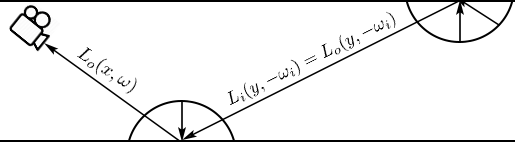
\includegraphics[width=0.7\textwidth]{images/rendering_equation.png}    
\end{center}
\caption{A diagrammatic representation of the recursive nature of the rendering equation. The outgoing radiance ($L_o$) in a given direction $\omega$ from a point $x$ requires an estimation of the incident radiance coming from all angles in the hemisphere around the point, that is $L_i(h(x, \omega_i),-\omega_i) = L_i(y_i, -\omega_i)$ $\forall \omega_i \in \Omega$. To calculate $L_i(y_i, -\omega_i)$ is identical to calculating the outgoing radiance $L_o(y_i, -\omega_i)$ as we assume no radiance is lost along a ray line, hence the $L_o$ is a recursive function. }
\label{fig:recursive_rendering}
\end{figure}

The $f_r$ term in Equation \ref{eq:rendering_equation} is known as the bidirectional reflectance distribution function (BRDF). On a high level, the BRDF describes how a surface interacts with light and upholds the law of conservation of energy \cite{glassner2014principles}. Every surface has a BRDF which determines when a ray intersects with that surface at a given incident direction, the probability distribution over the set of angles the ray can be reflected in. Therefore, querying the BRDF for a surface at point $x$ with incident ray direction $\omega'$ and given reflected direction $\omega$, that is $f_r(\omega', x , \omega)$,  a single scalar probability value is returned. This probability represents how likely a ray is to be reflected in direction $\omega$. A diffuse and specular surfaces BRDF's are depicted in \ref{fig:brdfs}. An example of a diffuse material is paper, as it reflects light almost equally in all directions for any angle of incidence. Whilst for specular materials, many metals exhibit specular reflections, where incident rays are reflected in a narrow area around the perfect reflection direction.

\begin{figure}[h]
\centering
\minipage{0.32\textwidth}
  
\includegraphics[width=\textwidth]{images/diffuse_brdf.png}   
  \subcaption{Diffuse BRDF}\label{fig:diffuse_brdf}
\endminipage\hspace{5em}
\minipage{0.32\textwidth}
  
\includegraphics[width=\textwidth]{images/specular_brdf.png}
  \subcaption{Specular BRDF}\label{fig:specular_brdf}
\endminipage
\caption{A representation of both a diffuse surface and specular surface BRDF for a given angle of incidence $\omega'$. The surface point is located where all end of the arrows converge. The arrows indicate a subset of direction possible for the incident ray to be reflected in. All possible directions reflected directions for a ray are defined between the surface point and the line , for an incident direction $\omega'$. The further away a point is on the line, the more likely a ray is to reflected in a direction from the surface point to that point on the line. The diffuse surface is equally likely to reflect a ray in any direction. Whereas, the specular surface favour a small subset are of direction in the hemisphere surrounding the surface point.}
\label{fig:brdfs}
\end{figure}

Another way to think about diffuse and specular materials is do they change in appearance depending on the viewing angle? For example, surface of paper appears to be identical no matter the viewing angle, however a shiny metal ball would appear to reflect what was in front of it which changes depending on the viewing angle, just like a mirror. These differences can be scene in Figure \ref{fig:material_pics}.

\begin{figure}[h]
\centering
\minipage{0.32\textwidth}
  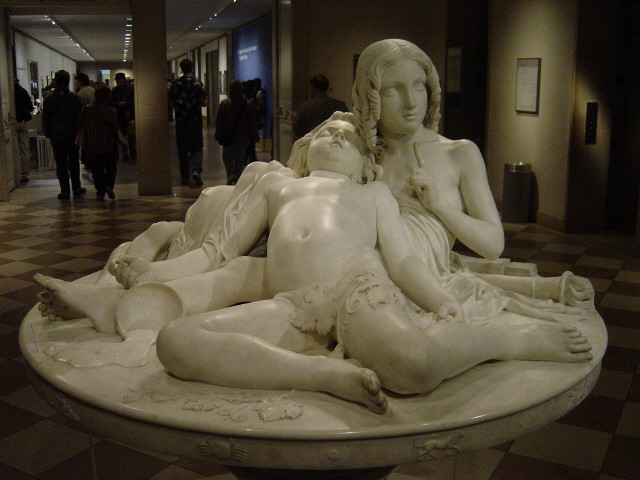
\includegraphics[width=\textwidth]{images/diffuse_sculpture.jpeg}   
  \subcaption{La Table aux Amours, Marble Sculpture}
\endminipage\hspace{5em}
\minipage{0.32\textwidth}
  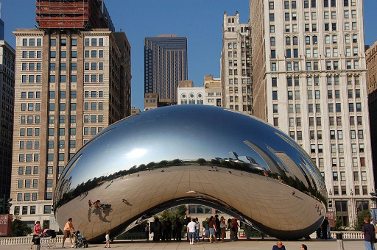
\includegraphics[width=\textwidth]{images/specular_sculpture.jpg}
  \subcaption{Cloud Gate, Stainless Steel Sculpture}
\endminipage
\caption{Two sculptures, one made from a diffuse material (left) and the other from a specular material.}
\label{fig:material_pics}
\end{figure}


A scene comprising of only diffuse materials is generally more computationally expensive to simulate, as one has to simulate rays reflecting in all directions around intersections points with surfaces, compared to a specular scene where only a small subset of directions need to be sampled for each intersection. So, from here on whenever a surface or BRDF is mentioned, assume it is diffuse as my descriptions can be extended to specular materials by restricting ray reflections to a limited set of angles.\\

Finally, as mentioned $cos(\theta_i)$ is the cosine of the angle $\omega_i$ between the normal of the point of the surface intersected with and the angle of incidence. The normal of a surface is the normalized vector that is perpendicular to the surface \cite{normals}. The $cos(\theta_i)$ is a weighting for reflected radiance from a point, where the larger the angle from the normal the smaller the reflected radiance. This simulates how light is spread across the surface, causing less light to be reflected in a direction which is further away from being perpendicular to the surface.

\subsection{Path Tracing}

In section \ref{sec:conceptual_path_trace} I already gave a high level overview of the how the path tracing algorithm where many light paths are sampled which consist of shooting a ray from the camera, through a pixel and into the scene to calculate a colour estimate. A pixels colour is then determined by averaging all light paths colour estimates. However I did not detail how to get the colour estimate of a light path. This is exactly what the solution to the rendering equation gives, as $L_o(x,\omega)$ gives the outgoing radiance for each sampled light paths initial direction $\omega$ and intersection point $x$. The radiance is then converted into a pixel colour value. Put another way, $L_o(x,\omega)$ is a pixels colour value where $\omega$ is the direction of the ray when shot from the camera, through the pixel and into the scene. Then $x$ is the position in the scene the ray first intersects with. \\

But how does one solve the rendering equation, as often it cannot be done analytically? This is what Monte Carlo integrating in path tracing is used for. Path tracing solves a slightly different form of the rendering equation to that in \ref{eq:rendering_equation}. To calculate the reflected radiance at point $x$ in the scene for the angle of incidence $\omega$, it is possible to instead calcualte the integral of all light paths which start at the intersection $x$ and reflect round the scene until a light source is intersected with. The proof behind this is detailed in \cite{stanford_graphics}, but conceptually it is simple. Previously the reflected radiance for $(x, \omega)$ was given by the integral of the incident radiance on $x$ with respect to the angle of incidence. To calculate this integral one can trace infinitely rays from the intersection point $x$ in all possible directions $\Omega$ until they high with a light source, the sum of which gives the total amount of incident light on point $x$. Therefore, path tracing solves a variant of the rendering equation to estimate $L_o(x, \omega)$ by integrating over all possible light paths starting from $x$ with respect to the surfaces intersected with. It is this integral which is solved via Monte Carlo integration, the details of which are given in Equation \ref{eq:rendering_eq_monte_carlo}.

\begin{equation}
\label{eq:rendering_eq_monte_carlo}
\begin{array}{l}
    L_o^N(x, \omega) = \frac{1}{N} \sum_{k = 0}^{N-1} L_e(x_0, \omega_0) + (L_i(x_1, -\omega_1) \cdot f_s(\omega_1, x_1, \omega_0) \cdot cos(\theta_{\omega_1})) / \rho_1\\ 
    \\
   \text{Such that}\\
   \\
    L_i(x_i, -\omega_i) = \begin{cases}L_e(x_i, \omega_i) + (L_i(x_{i+1}, -\omega_{i+1}) \cdot f_s(\omega_{i+1}, x_{i+1}, \omega_i) \cdot cos(\theta_{\omega_{i+1}})) / \rho_i & \mbox{if } x_i = \mbox{Light Source}\\ L_e(x_i, \omega_i) & \mbox{otherwise} \end{cases} 
\end{array}
\end{equation}
Where:
\begin{conditions}
 x_i   & Intersection location of the light path after $i$ reflections in the scene\\
 \omega_i   & Direction of the light path after $i$ reflections in the scene\\
 \rho_i   & Probability density function over reflected ray directions for position $x_i$ and $\omega_i$ angle of incidence
\end{conditions}

In Equation \ref{eq:rendering_eq_monte_carlo} recursive $L_i$ is still present, but the recursion is terminated when the light path intersects with a light source. By the law of large numbers in Equation \ref{eq:law_large_numbers}, the larger the number of sampled light paths ($N$), the closer each pixels approximation will be to the pixels true value as a result of solving the rendering equation. As known from section \ref{sec:rendering_equation}, the rendering equation follows the physical law of energy conservation, and due to this it accurately models light transport simulation for global illumination. Therefore, the more samples used in the Monte Carlo approximation in Equation \ref{eq:rendering_eq_monte_carlo}, the lower the amount of noise in the image \cite{christensen2016path}. An example of this concept applied to a simple forward path tracer is shown in Figure \ref{fig:reduce_noise_spp_example}.

% Include figure of increasing sampling count leading to a reduction in variance which corresponds to a reduction in image noise from things like fireflies
\begin{figure}[h]
\begin{center}
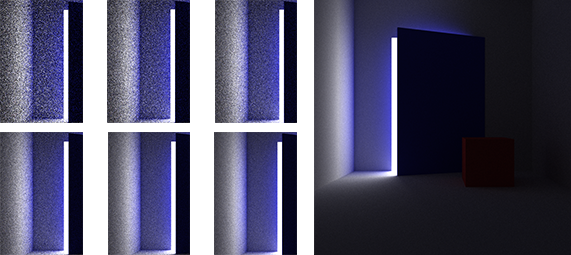
\includegraphics[width=0.99\textwidth]{images/renders/noise_reduction_default/increasing_samples.png}    
\end{center}
\caption{An indirectly illuminated scene from a default path tracer. The grid of image sections represent an increasing number of samples per pixel (SPP), beginning in the top left with 16 SPP, to the bottom right with 512 SPP. The full image on the right is a reference image with 4096 SPP where the Monte Carlo approximation has almost converged for pixel values.}
\label{fig:reduce_noise_spp_example}
\end{figure}

Algorithm \ref{alg:forward_path_tracing} describes a forward path tracer which computes one sample inside the summation of Equation \ref{eq:rendering_eq_monte_carlo} to find a sampled light paths colour estimate for a given pixel. To render an entire image, this algorithm would be called for each pixel $N$ times (where $N$ is the number of samples per pixel) and the colour estimates of all $N$ rays would be average to find the colour estimate of the pixel.\\

\begin{algorithm}[H]
\label{alg:forward_path_tracing}
\SetKwProg{Fn}{Function}{ }{end}
\SetAlgoLined
 \Fn{pathTrace(camera, scene, pixel)}{  
   $throughput \leftarrow 1$\\
   $ray \leftarrow initialiseRayForPixel(pixel, camera)$\\
    \For{$i = 0$ \KwTo $\infty$}{
        $(y, norm) = closestIntersection(ray, scene)$\\
        \If{$noIntersection(y)$}{
            \Return $throughput \cdot \text{environmentLightRadiance}(ray,y)$
        }
        \ElseIf{$areaLightIntersection(y)$}{
            \Return $throughput \cdot \text{areaLightRadiance}(ray, y)$
        }
        $(\omega, \rho_i, f_s) \leftarrow \text{sampleRayDirRandomly(y)}$\\
        $throughput \leftarrow throughput \cdot f_s \cdot cos(norm, \omega) / \rho_i$\\
        $ray \leftarrow (y,\omega)$
    }
 }
 \caption{Forward path tracer}
\end{algorithm}

As path tracing is a Monte Carlo method for solving the rendering equation, Importance sampling can be applied in order to reduce the variance pixel colour estimates. In section \ref{sec:importance_smapling} it was shown that by using a probability density function ($pdf$) which closely matches the shape of the function being integrated, the variance in the Monte Carlo estimate is significantly reduced. Applying this to Equation \ref{eq:rendering_eq_monte_carlo}, the term $\rho_i$ which represents the probability density function for sampling the next ray direction at intersection location $x_i$ with angle of incidence $\omega_i$. Currently you can assume that the probability density function $\rho_i$ is uniform. But this can be modified with prior knowledge regarding which directions are more important for continuing a light path in, where an important direction is one which leads to a high contribution of radiance to the pixel estimate.\\

The question now is, can one have any knowledge for which directions contribute the most radiance to the pixels colours value? The answer is yes, and there has been a large amount of research in this which resides in the topic of light transport simulation. The simplest example lies within the rendering equation itself, $cos(\theta_i)$. As previously discussed, this term acts as a weighting for the radiance contribution of outgoing light paths. So, the probability density function $\rho_i$ can also be weighted by $cos(\theta_i)$, which is likely to reduce the pixel value variance. There exists many other methods of retrieving knowledge from the scene to use in importance sampling during rendering. For example, irradiance cahcing \cite{bashford2012significance}, table-driven adaptive importance sampling \cite{cline2008table}, and sequential Monte Carlo adaptation \cite{pegoraro2008towards}. However as discussed in section \ref{sec:motivation}, these previous methods do not effectively reduce the number of zero contribution light paths, meaning their ability to image noise for certain scenes is very limited. Instead, Nvidiai proposed that reinforcement learning can be used for this \cite{dahm2017learning} which is the main inspiration for my work. In the proceeding sections I will discuss in detail how it is possible to apply reinforcement learning for importance sampling in light path construction.

\section{Reinforcement Learning and TD-Learning}
Now that it is clear how Importance sampling light paths can be used to reduce variance in Monte Carlo path tracing, it is time to introduce the concept of reinforcement learning as I will be using this to gain knowledge for this Importance sampling. This section aims to give a quick introduction to reinforcement learning and TD-learning to cover all of the background material of the learning methods I will be using, before describing how they are applied to path tracing in the next section.

\subsection{Markov Decision Processes}
Reinforcement learning is one of the three archetypes of machine learning and it is concerned with finding what action should be taken in a given situation, in order to maximise a numerical reward \cite{sutton2011reinforcement}. This problem is formalized by a finite Markov Decision Process (MDP), which is designed to capture the most important aspects of the problem a learning agent faces when interacting over time with its environment to achieve a goal. A MDP is summarised in \ref{fig:mdp} and can be described in terms of the following:

\begin{itemize}
\item \textbf{Agent} - The learner and decision maker which takes an action $A_t$ in an observed state $S_t$ (where $t$ is the current time step), receiving an immediate numerical reward $R_{t_+1}$ and the next observed state $S_{t+1}$
\item \textbf{Environment} - What the agent interacts with when taking an action $A_t$ in state $S_t$ and produces both $R_{t+1}$ \& $S_{t+1}$ 
\end{itemize}

\begin{figure}[h]
\begin{center}
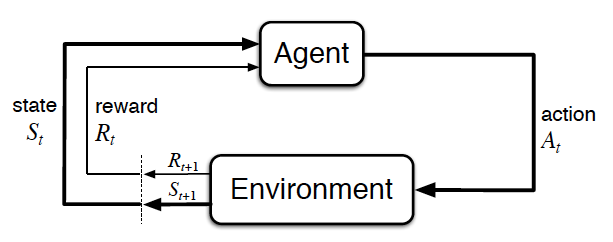
\includegraphics[width=0.5\textwidth]{images/MDP.png}    
\end{center}
\caption{Markov Decision Process \cite{sutton2011reinforcement}}
\label{fig:mdp}
\end{figure}

\noindent
An MDP comprises of the following the following tuple:

$$(\mathcal{S}, \mathcal{A}, p,\gamma)$$
Where:
\begin{conditions}
\mathcal{S}   &  The set of all states\\
\mathcal{A}   &  The set of all actions\\
p   & Probability of receiving reward $r$ and state $s'$ when in the previous state $s$ and action $a$ was taken\\
\gamma   & The discount factor which makes the agent value immediate rewards higher than later ones \\
\end{conditions}

\noindent
An important detail of an MDP which makes it far easier to implement in practice is that any problem modelled by an MDP assumes the Markov property.

\begin{quote}
"The future is independent of the past, given the present." - \textit{Hado van Hasselt, Senior Research Scientist at DeepMind} \cite{introToRL}
\end{quote}

This is expressed mathematically for an MDP in equation \ref{eq:markov_property}. Put simply, the Markov property means the current state captures all relevant information from the history of all previous states the agent has experienced, meaning the history is not needed.

\begin{equation}
\label{eq:markov_property}
p(R_{t+1} = r, S_{t+1} = s' | S_t = s) = p(R_{t+1} = r, S_{t+1} = s' | S_1, .. , S_{t-1}, S_{t})
\end{equation}

\subsection{Goals and Rewards}
The goal thought of for a reinforcement learning agent can change significantly depending on the problem, for example in the case of a game it may be to maximise the total score in one play-through. Or for a robotic space rover it may be to discover the most amount of unseen terrain. However, in terms of an MDP all AI agents goals a described as maximising the total amount of cumulative reward received. This is more formally described by the reward hypothesis \cite{sutton2011reinforcement}

\begin{quote}
Any goal can be formalized as the maximisation of the expected value of the cumulative sum of a received scalar reward signal.
\end{quote}

Once again in the case of an agent learning the best possible action to take for any state in the game (known as the optimal policy), a reward signal could be the points gained by making a certain move. Therefore, to maximise the expected return would be to maximise the number of points received in a play-through.  The return is formally defined in Equation \ref{eq:return} in terms of a reward sequence combined with the discount factor, which as previously mentioned trades off later rewards for more immediate ones. If a discount factor ($\gamma$) is closer to 1 the agent is said to be far sighted, as it gives future rewards a high weighting. Whereas a myopic agent is one which has a discount factor closer closer to 0, as it gives a lower weighting to future rewards for their contribution towards the return $G_t$ \cite{introToRL}. 

\begin{equation}
\label{eq:return}
G_t = R_{t+1} + \gamma R_{t+2} + \gamma^2 R_{t+3} + ... = \sum^\infty_{k=0} \gamma^k R_{t+k+1}
\end{equation}

This formulation works well if the agents interactions with the environment break down easily into sub-sequences \cite{sutton2011reinforcement}, where an agent starts in one of a given set of starting states and takes a series of actions to reach a terminal state. From the terminal state the agent can be reset to one of the starting states to begin learning once again. This applies to path tracing, where the terminal state is one in which the light path has intersected with a light, but this will be discussed in detail in Section \ref{sec:td_light_transport}.

\subsection{Value Function and Optimality}
All reinforcement learning algorithms I will be considering involve the concept of a value function. There are two kinds of value functions, one which determines the value of being in a given state, the other determines the value of being in a certain state and taking a certain action, known as a state-action pair. The methods I consider are those which use state-action pair value functions, where the value of a state-action pair is defined in terms of the expected return from that state-action pair.

An agent follows a policy $\pi$, which determines how the agent will act in a given state. Formally, a policy is a mapping from states to probabilities of selecting a particular action. When an agent is following policy $\pi$ at time $t$, then $\pi(a|s)$ is the probability that $A_t = a$ if $S_t = s$. Reinforcement learning algorithms state how an agents policy changes from experience. 

The value of a state-action pair $(s,a)$ under a policy $\pi$, is given in Equation \ref{eq:value_function} denoted as $q_\pi(s,a)$,. This value function is commonly known as the action value function for policy $\pi$. Stating 'under policy $\pi$' is important as the value of a given state-action pair depends upon the actions we take onwards from taking action $a$ in state $s$ due to $\pi$. $\mathbf{E}_\pi$ denotes the expected value of a random variable, given that the agent follows policy $\pi$. From this, if one were to keep track of the actual returns received for taking a state-action pair, then as the number of times the state-action pair is chosen tends to infinity, the average of the returns will converge on the true expected value of the return for the state-action pair $q_\pi(s,a)$.

\begin{equation}
\label{eq:value_function}
q_\pi(s, a) = \mathbf{E}_\pi[G_t | S_t = s, A_t = a] = \mathbf{E}_\pi [\sum_{k=0}^{\infty} \gamma^k R_{t+k+1} | S_t = s, A_t = a]
\end{equation}

Now, if you had an AI agent the best way it could perform would be to maximise the expected reward it receives in an episode. In terms of a policies, this is know as the optimal policy which is said to be better then all other policies and agent can follow. Formally, the optimal policy is $\pi$ if $\pi \geq \pi'$ for al possible policies $\pi'$. Where, $\pi \geq \pi'$ if and only if $q_\pi(s,a) \geq q_{\pi'}(s,a)$ for all $s \in \mathcal{S}$ and $a \in \mathcal{A}$. The optimal policy is denoted as $\pi_*$ and the value function following the optimal policy, which is the optimal value function, is denoted $q_*(s,a)$. The optimal value function is defined in Equation \ref{eq:optimal_value}.

\begin{align}
q_*(s,a) & = \max_\pi q_\pi(s,a) \label{eq:optimal_value} \\
 & = \mathbf{E}[R_{t+1} + \gamma \max_{a'} q_* (S_{t+1}, a') | S_t = s, A_t = a]  \label{eq:bellman_optimal}
\end{align}

Equation \ref{eq:bellman_optimal} defines the Bellman optimality equation, which states that the value of a state-action pair under an optimal policy must be equal to the expected return of the immediate reward plus the highest valued state-action pair available from the next state. Intuitively, if the optimal policy is available which is essentially a cheat sheet of what action is most valuable to take in each state. Then the value of a given state-action pair should be equal the immediate reward received by taking the action in the current state, plus the value of the best action to take in the next state given by the cheat sheet/optimal policy. Therefore, if one has the optimal value function, the optimal policy can easily be found by maximising the choice of action $a$ for $q_*(s,a)$  in state $s$ \cite{sutton2011reinforcement}. \\ 

To summarize, the aim from here on is to build an agent which is able to learn the optimal value function, but whilst this is provably possible, it rarely happens in practice. However, the learning methods I will discuss in the next section on TD-learning are able to find a good value function for light path direction sampling.

\subsection{Temporal Difference Learning}

TD-Learning is combination of Monte Carlo and Dynamic Programming reinforcement learning methods for learning the optimal value function from equation \ref{eq:optimal_value}. I will not discuss the details of Monte Carlo and Dynamic Programming methods as they are not investigated as part of my work. However, the reasoning for choosing to study  TD-learning approaches over these two alternative approaches are as follows; TD-learning can perform learning updates of the value function throughout an episode, unlike Monte Carlo approaches which wait until the end \cite{model_free_prediction}. This means TD-learning algorithms can be written in an online learning algorithm \cite{sutton2011reinforcement}. TD-learning can learn directly from experience, as it does not require a true model of the environment in order to learn, unlike Dynamic Programming methods \cite{mdp_dynamic_prog}. This means TD-learning is model-free, avoiding the expense of building the true model of the environment. I will now introduce

I will now introduce three different temporal difference learning methods which are required knowledge for the rest of my work.

\subsubsection*{Sarsa}

Sarsa is a on-policy TD method which learns a good state-action pair valuation function $q_\pi(s,a)$. The Sarsa learning rule is presented in Equation \ref{eq:sarsa}, and I have chosen to present this method first to explain some key concepts TD-learning methods share. Firstly, $Q$ denotes the current value function under policy $\pi$, $q_\pi$. Therefore the left arrow indicates an update in the value of the current estimate $Q$. Also notice, how the current estimate is update upon every time step $t$, this means Sarsa like other TD-learning methods can learn during an episode as previously mentioned. The $\alpha$ term is the current learning rate where $\alpha \in [0,1]$ and $\gamma$ is the discount factor as previously discussed. Finally, Sarsa performs what is known as bootstrapping in the context of reinforcement learning \cite{sutton2011reinforcement}. Bootstrapping is where the  estimate of the valuation function ($Q$), is updated based on some new data by experience, which is the immediate reward $R_{t+1}$. As well as, the current estimate of the valuation function $Q$. Sarsa therefore learns from experience, whereby an action is $A_t$ is taken in state $S_{t}$, leading to an immediate reward $R_{t+1}$ which is used to update the current estimate $Q$.

\begin{equation}
Q(S_t, A_t) \leftarrow Q(S_t, A_t) + \alpha[R_{t+1} + \gamma Q(S_{t+1}, A_{t+1}) - Q(S_t, A_t)]
\label{eq:sarsa}
\end{equation}

The reasoning behind the name Sarsa is that the method uses every element in the quintuple of events, $Q(S_t, A_t, R_{t+1}, S_{t+1}, A_{t_1})$, which makes up a transition between each time step of state-action pairs. Sarsa is an on-policy TD-learning method, as to choose the next action to take in the next state ($Q(S_{t+1}, A_{t+1}$) the policy is used. \\

To make Sarsa learning and TD-learning in general more concrete, imagine a robot with a camera whose goal it is to manoeuvre to the end of a corridor. Each time step is the point when a new frame is rendered on the camera, and the state is the image displayed by the camera. The robots actions consist of moving a short distance in a set of four different direction. If the robot were to learn using Sarsa, the robot would have a large table storing the value of each state-action pair $Q(S_t, A_t)$, which represents the current value function. The robot would then select an action at each time step according to the policy $\pi$ to receive a reward signal based on its distance to the end of the corridor. The robot would then perform a lookup on the large table indexing with the action it took in the state it was in and perform the update rule in \ref{eq:sarsa}. This large table representing the current estimate of the optimal value function is also know as a Q-table, where each value in the table is known as a Q-value, $Q(S_t, A_t)$. By following a suitable policy, the robot will over time will keep updating its Q-values to improve
its estimate of $q_\pi(s,a)$.

\subsubsection{Q-Learning}

Q-learning is very similar to Sarsa except it is an off-policy TD-learning algorithm. Also, if all state-action pairs are visited infinitely many times, it is proven that Q-learning can converge on the optimal policy $q_\pi(s,a)$, therefore it is generally a preferred method. The learning rule is displayed in Equation \ref{eq:q_learning}, where rather then following a policy $\pi$ to select the action to update with, the maximum value of the highest valued action in the next state is selected ($\max_a Q(S_{t+1}, a$). This means the agent following policy $\pi$ will still choose its actions in a state based on $\pi$, however when it update its valuation function $Q$, the action chosen to update with may not necessarily be the same as the action chosen. Hence, Q-learning is an off-policy TD-learning algorithm.

\begin{equation}
Q(S_t, A_t) \leftarrow Q(S_t, A_t) + \alpha[R_{t+1} + \gamma \max_aQ(S_{t+1}, a) - Q(S_t, A_t)]
\end{equation}

\subsubsection{Expected Sarsa}

Expected Sarsa is a TD-learning algorithm which is generally found to be superior to both Q-learning and Sarsa in practice \cite{sutton2011reinforcement}. It is very similar to Q-learning, but instead of using the maximum value of the next state-action pairs it takes the expected value over them. This means Expected Sarsa takes into account how likely each action is under the current policy as shown in Equation \ref{eq:expected_sarsa}. Where $\pi(a | S_{t+1})$ returns the probability of selecting action $a$ in state $S_{t+1}$, while following the policy $\pi$. Note, Expected Sarsa may be used as either an on-policy of off-policy algorithm, for example if the policy $\pi$ was set to the greedy-policy used in Q-learning, the learning rule would become identical to that of Q-learning. Therefore, Expected Sarsa generalizes over Q-learning. Expected Sarsa also reduces the variance in the value function approximation compared to that of Sarsa, as the expectation taken over the current valuation estimate for state-action pairs used.

\begin{align}
Q(S_t, A_t) &  \leftarrow Q(S_t, A_t) + \alpha [R_{t+1} + \gamma \mathbf{E}[Q(S_{t+1}, A_{t+1}) | S_{t+1}] - Q(S_t, A_t)]\\
 & \leftarrow Q(S_t, A_t) + \alpha [R_{t+1} + \gamma \sum_a \pi(a| S_{t+1}) Q(S_{t+1}, a) - Q(S_t, A_t)]
 \label{eq:expected_sarsa}
\end{align}

\subsection{Exploration vs Exploitation}

Up to now I have formally introduced what reinforcement learning is, including what the optimal value function is and different ways to learn it. As for the TD-learning methods presented so far, I have not discussed any details about the kind of policy an agent should use to select actions in the process of learning. Deciding on this policy is very influential on our agents performance, as the agent needs to gather enough information about its environment to make the best overall decisions. Therefore, online decision-making requires a fundamental choice to be made by the agent every time it chooses to take an action \cite{exploration_vs_exploitation}. This is between the following:

\begin{itemize}
\item \textbf{Exploration}: Maximise the agents performance based on the current knowledge available
\item \textbf{Exploration}: Gain more knowledge about the environment
\end{itemize}

This means a good learning strategy for an agent may be to sacrifice short-term performance to maximise it in the long-term. This applies directly to the policy used in TD-learning methods. Initially exploration is the most important to quickly gain a broad amount of knowledge about the environment and opening up more specific areas for further exploration. Then over time the policy should favour exploitation more and more by taking known higher valued actions. An example of this kind of policy is the decaying $\epsilon$-greedy policy \cite{sutton2011reinforcement}. This policy maintains the current value of $\epsilon \in [0,1]$ and involves sampling a random number $x \in [0,1]$, then if $x > \epsilon$ exploitation occurs, else exploration. By exploitation it is common practice to choose the current highest valued action, whereas exploration involves choosing one at random. Overtime $\epsilon$ is decreased to match the behaviour of increasing exploitation as more knowledge is gained.

\section{Linking TD-Learning and Light Transport Simulation}
\label{sec:td_light_transport}
With TD-learning learning introduced, I will now link TD-learning to light transport simulation for importance sampling light path directions. Specifically, due to the benefits discussed of Expected Sarsa over Q-learning and Sarsa, I will represent the rendering equation as an Expected Sarsa learning rule. This was orginally introduce by Nvidia in 2017 \cite{dahm2017learning}. 

First, the Expected Sarsa learning rule's summation over the set of all actions $\mathcal{A}$ can be represented as an integral with respect to an action $a$, as shown in Equation \ref{eq:sarsa_integral}. This implies the action space is continuous:

\begin{align}
Q(S_t, A_t) & \leftarrow Q(S_t, A_t) + \alpha [R_{t+1} + \gamma \sum_a \pi(a| S_{t+1}) Q(S_{t+1}, a) - Q(S_t, A_t)]\\
& =  (1 - \alpha) \cdot Q(S_{t},A_t) + \alpha \cdot \left( R_{t+1} + \gamma \sum_a \pi(a|S_{t+1}) Q(S_{t+1}, a) \right)\\
& = (1 - \alpha) \cdot Q(S_{t},A_t) + \alpha \cdot \left( R_{t+1} + \gamma \int_\mathcal{A} \pi(a|S_{t+1}) Q(S_{t+1}, a) da \right)
 \label{eq:sarsa_integral}
\end{align}

Recall the rendering equation from section \ref{sec:rendering_equation} describes the radiance in an outgoing direction $\omega$ from point $x$ is equivalent to the emitted radiance in the direction plus the reflected radiance in the direction. 

\begin{equation}
L_o(x, \omega) = L_e(x,\omega)  + \int_\Omega L_i(h(x, \omega_i), -\omega_i)  \cdot f_r(\omega_i, x, \omega) \cdot \cos(\theta_i) d\omega_i \nonumber
\end{equation}

\noindent
Now, by matching  terms from the rendering equation to the Expected Sarsa learning rule in Equation \ref{eq:sarsa_integral}, Equation \ref{eq:expected_sarsa_td_learning} is formed. Where this new learning rule is designed to approximate the outgoing radiance in direction $\omega$ from point $x$. Therefore, the value of the state-action pair $Q(x = S_t, \omega = A_t)$ is determined by the amount of radiance incident in direction $\omega$ from point $x$. An important detail which may be overlooked is that the substitution of $\gamma \cdot \pi(a|S_{t+1})$ for $f_s(\omega_k, y, -\omega) \cdot \cos(\theta_i)$ ensures that a trade off of long term rewards for more immediate rewards is made as $f_s(\omega_k, y, -\omega) \cdot \cos(\theta_i) \leq 1$. Meaning, the learning rule accurately accounts for a light paths loss of energy as reflects off surfaces in the scene.

The following lists what each term in the Expected Sarsa learning rule is matched to:
\begin{conditions}
 S_t &  3D position in the scene, $x \in \mathbb{R}^3$  \\
 
 A_t & Sampling a direction to continue the light path from location $x$, in direction $\omega$ \\   
 
S_{t+1}   &  3D position of a light ray from reflected from $x$ in direction $\omega$, $y = h(x, \omega)$ \\

R_{t+1} & Emitted radiance from point $y$ in direction $-\omega$, $L_e(y, -\omega)$\\

\mathcal{A} & All direction in the hemisphere at $x$, oriented to the surface normal at $x$, $\Omega$\\

\gamma \cdot \pi(a|S_{t+1}) & BRDF and the cosine of the angle $y, \omega_i$, $f_r(\omega_i, y, \omega) \cdot \cos(\theta_i)$\\
    
Q(S_t, A_t) & Radiance incident on $x$ from direction $\omega$, $-L_i(x, \omega) = Q(x, \omega)$\\
\end{conditions}

\begin{equation}
Q(x, \omega) \leftarrow (1 - \alpha) \cdot Q(x, \omega) + \alpha \cdot \left( L_e(y, -\omega) + \int_\Omega Q(y, \omega_i) f_s(\omega_i, y, -\omega) \cos(\theta_i) d\omega_i \right)
\label{eq:expected_sarsa_td_learning}
\end{equation}

Finally, Monte Carlo integration with a uniform distribution for the probability density function can be used to approximate the integral in Equation \ref{eq:expected_sarsa_td_learning}. This converts the action space from continuous to $n$ discrete angles and provides a numerical solution for approximating the outgoing radiance from $x$ in direction $\omega$, which is presented in Equation \ref{eq:mc_expected_sarsa_td_learning}.

\begin{equation}
Q(x, \omega) \leftarrow (1 - \alpha) \cdot Q(x, \omega) + \alpha \cdot \left( L_e(y, -\omega) +\frac{2 \pi}{n} \sum_{k=1}^{n-1} Q(y, \omega_k) f_s(\omega_k, y, -\omega) \cos(\theta_k)  \right)
\label{eq:mc_expected_sarsa_td_learning}
\end{equation}

To summarize, I have derived a learning rule for determining the outgoing radiance from a position in a given direction $Q(x, \omega)$. In the context of reinforcement learning this is an approximate value function $Q$, which attempts to approximate the true value function $q_*(s,a)$. So for light transport, the optimal value function $q_*(x, \omega)$ would be the true value of radiance outgoing from point $x$ in direction $\omega$. The purpose of approximating the radiance $Q(x, \omega)$ is to use this as knowledge for importance sampling ray directions in path tracing to avoid zero-contribution light paths. Exactly how this is done is specified in the next section \ref{sec:expecte_sarsa_path_tracer}.

\section{The expected Sarsa Path tracer}
\label{sec:expecte_sarsa_path_tracer}
Monte Carlo Integration, importance sampling, Monte Carlo path tracing, reinforcement learning and the link between temporal difference learning and light transport have all been introduced. So now it is finally time to combine all of these concepts by introducing Nvidia's Expected Sarsa path tracer which uses the learning rule derived in \ref{eq:mc_expected_sarsa_td_learning} for Importance sampling. This method progressively reduces the number of zero-contribution light paths sampled during rendering, reducing the variance in the Monte Carlo approximation of a pixels colour, reducing the noise in rendered images. 

\subsection{The Irradiance Volume}
The learning rule introduced in \ref{sec:td_light_transport} requires some sort of data-structure for looking up and updating the outgoing radiance at point $x$ in direction $\omega$, which from here on I will refer to as a Q-value. Therefore, the main requirement of the data structure is that it has some was of representing a discrete set of angles ($\omega_k$) in a hemisphere located at a position $x$ and oriented to the surface normal at $x$. The Irradiance Volume data structure \cite{greger1998irradiance} meets this requirement.\\

\begin{figure}[h]
\begin{center}
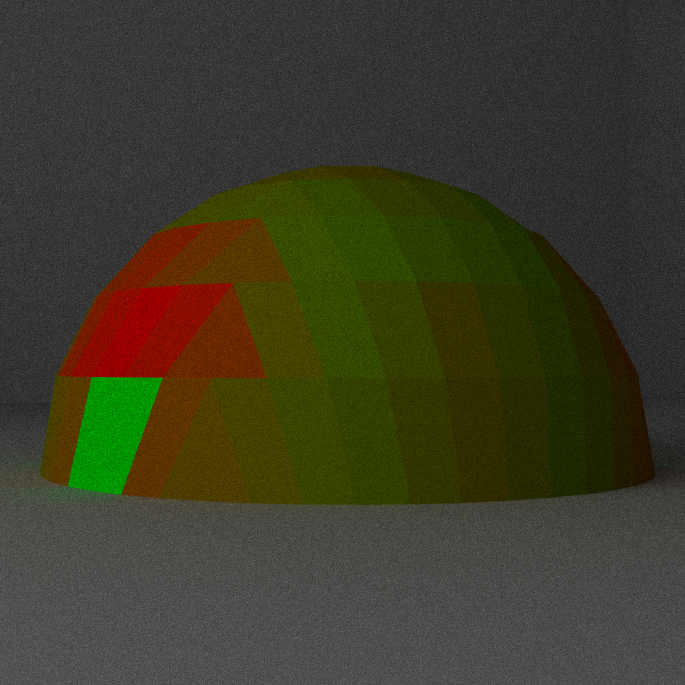
\includegraphics[width=0.3\textwidth]{images/renders/hemispheres/irradiance_volume.png}    
\end{center}
\caption{An Irradiance Volume. Each sector holds the incoming radiance $L_i(x,\omega_k)$, the more green a sector is the lower the stored radiance in that sector, the more red a sector is the higher the stored radiance in that sector. }
\label{fig:irradiance_volume}
\end{figure}

Originally designed to be used for pre-computation of radiance values which are looked up at runtime to approximate global illumination, the Irradiance Volume data structure is essentially a discretized version of a hemisphere which is visually represented in Figure \ref{fig:irradiance_volume}. The image shows the discrete sectors which make up a hemisphere, this was implemented by converting a 2D square grid into the 3D hemisphere shown, which is known as an adaptive quadrature. Where all sectors in the 2D grid have an equal area and a mapping introduced in \cite{shirley1994notes} converts the 2D grid coordinates into a regular discretized hemisphere in 3D space. The mapping ensures the hemisphere sectors remain equal to one another, meaning the discrete set of direction represented by the hemisphere are of equal angles apart from one another.\\

\begin{figure}[!htb]
\centering
\minipage{0.32\textwidth}
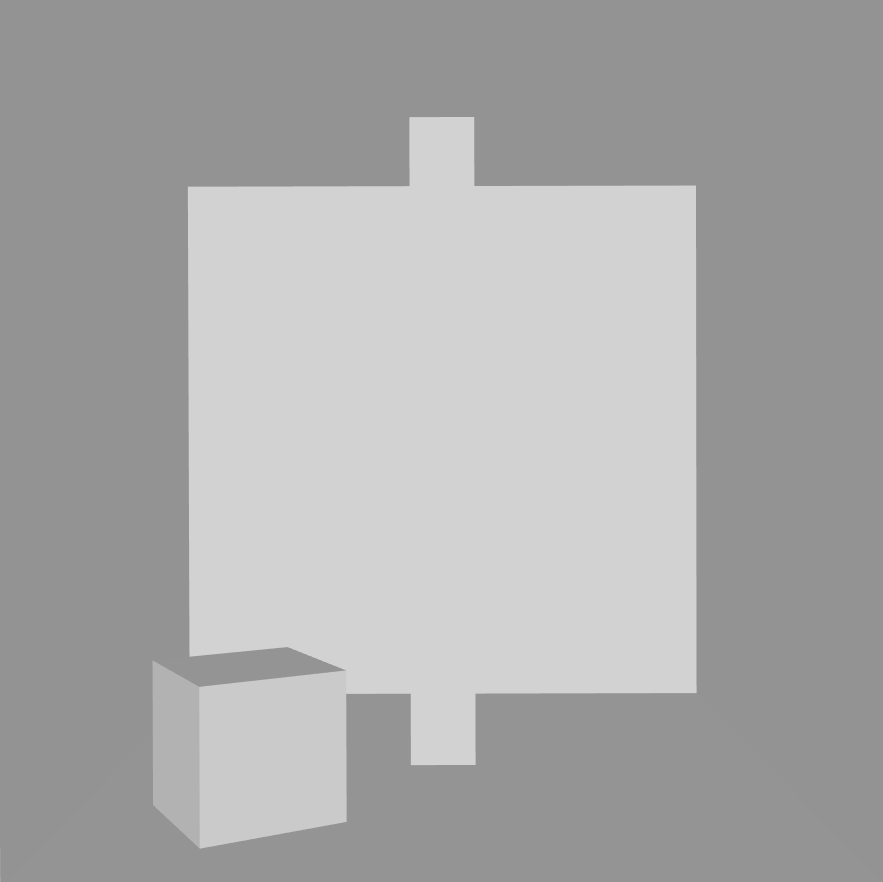
\includegraphics[width=1\textwidth]{images/renders/simple_room/geometry.png}
  \subcaption{Representation of the scenes geometry meshes}
\endminipage\hfill
\minipage{0.32\textwidth}
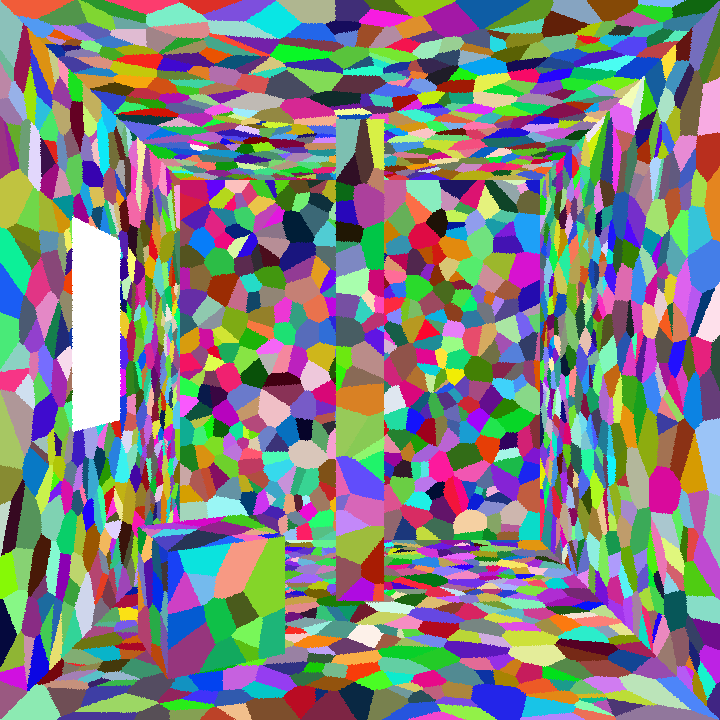
\includegraphics[width=1\textwidth]{images/renders/simple_room/voronoi.png}
   \subcaption{Voronoi Plot of Irradiance Volume locations}
\endminipage\hfill
\minipage{0.32\textwidth}
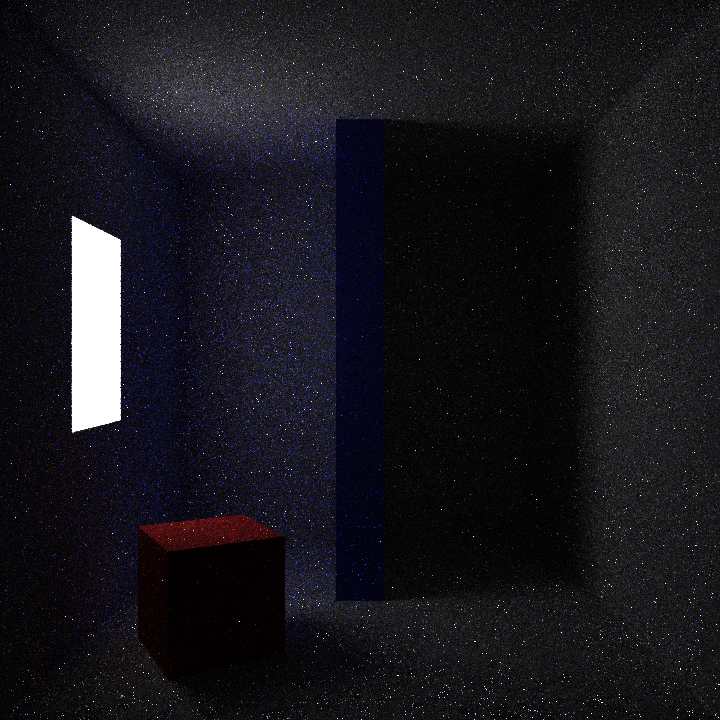
\includegraphics[width=1\textwidth]{images/renders/simple_room/reinforcement_16.png}
  \subcaption{Expected Sarsa path tracer with 16 SPP}
\endminipage
\caption{An example of discretizing location in the scene into Irradiance Volume locations. The geometry mesh (a) is used to uniformly sample Irradiance volume positions. Image (b) shows a voronoi plot for the Irradiance Volumes in the scene, where each pixel is coloured to the represent its closest Irradiance Volume, so each sector of colour in (b) represents a different Irradiance Volume location. Finally (c) gives a render using the Expected Sarsa path tracer based on Algorithm \ref{alg:expected_sarsa_pathtracer}.}
\label{fig:scene_discretization_example}
\end{figure}

Each sector of the Irradiance Volume is then used to store the current approximation of radiance from the centre of the hemispheres location $x$, in the outgoing direction formed by the unit vector from $x$ to the centre of the sector. Therefore, an Irradiance Volume stores the radiance (Q-value) for a given position $x$ (state) in each direction $\omega_k$ (action), for all sectors $k$ in the hemisphere located at $x$. In order to store Q-values across the scene, Irradiance Volumes can be uniformly sampled over the scenes geometry as shown in Figure \ref{fig:scene_discretization_example}. Then to lookup a radiance/Q-value for a given position $x$ in direction $\omega_k$, a nearest neighbour search is performed to find the closest Irradianc volume to position $x$, then retrieve the Q-value from the sector at index $k$. Giving a lookup and update time of $O(\log n) + O(1) = O(\log n)$ when using a data structure such as a KD-Tree for nearest neighbour search \cite{bentley1975multidimensional}. Lookup and update procedures from the Irradiance volumes in the scene is all that is needed to apply the Expected Sarsa learning rule in Equation \ref{eq:mc_expected_sarsa_td_learning}.

\subsection{Expected Sarsa Path Tracing}

\subsubsection{Algorithm}
The Expected Sarsa based path tracing algorithm is very similar to the original forward path tracer introduced in Algorithm \ref{alg:forward_path_tracing}. The algorithm learns online, meaning after every rendered frame pixel values are likely to have a lower variance due to a reduction in the number of zero contribution light paths. Initially radiance volumes are sampled uniformly across the room with all Q-values initialised to a small constant proportional to the number of sectors on each hemisphere $k$. This encodes the assumption that initially the radiance in all direction from any given point in the room is equal, as initially there is no prior knowledge of any radiance values $Q(x, \omega)$. With the radiance volumes set up, $n$ sampled light paths are traced through each pixel from the camera and into the scene. The average colour estimate of the $n$ sampled light paths per pixel is averaged to find the colour of each pixel, every rendered frame. The colour estimate of each sampled light path is found by Algorithm \ref{alg:expected_sarsa_pathtracer}. The two additions to this algorithm from the forward path tracer in Algorithm \ref{alg:forward_path_tracing}, are as follows:

\begin{enumerate}
\item Once the ray has intersected with a position in the scene $y$ from a position $x$, update the radiance estimate $Q(x, \omega)$ using the Expected Sarsa learning rule derived in Equation \ref{eq:mc_expected_sarsa_td_learning}. This is based on the light emitted from $y$ in direction $-\omega$ and the outgoing radiance estimate in direction $-\omega$ from point $y$ described by the summation. The summation involves summing all Q-values for the closest radiance volume to position $y$. Each of which are multiplied by BRDF of the surface at $y$, as well as the cosine of the angle between the sector direction for the Q-value ($\omega_k$) and the surface normal $y$.

\item The direction to continue the light path in is sampled proportional to the Q-values stored in the closest hemisphere to position $y$. This is achieved by normalizing the Q-values for the radiance volumes, converting them into a distribution which is appropriately known as the radiance distribution. Then inverse transform sampling \cite{devroye2006nonuniform} is performed to get a direction in the hemisphere to sample a ray in. Inverse transform sampling is where a random number $r \in [0,1]$ is sampled, then the largest number $x$ from the domain of the cumulative distribution $P(X)$ is returned where $ P(-\infty < X < x) \leq r$. 
\end{enumerate}

\begin{algorithm}[H]
\label{alg:expected_sarsa_pathtracer}
\SetKwProg{Fn}{Function}{ }{end}
\SetAlgoLined
 \Fn{pathTrace(camera, scene, pixel)}{  
   $throughput \leftarrow 1$\\
   $ray \leftarrow initialiseRayForPixel(pixel, camera)$\\
    \For{$i = 0$ \KwTo $\infty$}{
        $(y, norm) = closestIntersection(ray, scene)$\\
        \tcc{Addition (1)}
        \If{$i > 0$}{
            $Q(x, \omega) \leftarrow (1 - \alpha) \cdot Q(x, \omega) + \alpha \cdot \left( L_e(y, -\omega) +\frac{2 \pi}{n} \sum_{k=1}^{n-1} Q(y, \omega_k) f_s(\omega_k, y, -\omega) \cos(\theta_k)  \right)$
        }    
            
        \If{$noIntersection(y)$}{
            \Return $throughput \cdot \text{environmentLightRadiance}(ray,y)$
        }
        \ElseIf{$areaLightIntersection(y)$}{
            \Return $throughput \cdot \text{areaLightRadiance}(ray, y)$
        }
        \tcc{Addition (2)}
        $(\omega, \rho_i, f_s) \leftarrow \text{sampleRayDirProportionalToQ(y)}$\\
        $throughput \leftarrow throughput \cdot f_s \cdot cos(norm, \omega) / \rho_i$\\
        $ray \leftarrow (y,\omega)$
    }
 }
 \caption{Expected Sarsa forward path tracer \cite{dahm2017learning}}
\end{algorithm}

\subsubsection{Monte Carlo Integration}
It is important for the modified path tracing algorithm to converge to ensure consistency, meaning all introduced artefacts such as image noise are guarenteed to vanish over time \cite{dahm2017learning}. A decaying learning rate for $\alpha$ can be used to do so, see Equation \ref{eq:decay_lr}. Where $\text{i}(rv, \omega_k)$ is the number of times the rendering algorithm has updated the Q-value of the Irradiance Volume $i$ for sector $k$ representing angle $\omega_k$.

\begin{equation}
\label{eq:decay_lr}
\alpha(x, \omega) = \frac{1}{1 + \text{visits}(x, \omega_k)}
\end{equation}

Due to the importance sampling from addition (2), the probability density function over sampled directions $\omega$ at location $x$ is no longer uniform. Instead it is equal to the normalized Q-values for the closest Irradiance Volume to the point $x$. Therefore the evaluated probability density function $\rho_i$ must also take the shape of the probability distribution to correctly apply Monte Carlo Integration. To do so I have derived an Equation \ref{eq:mc_expected_sarsa_pdf} to determine the value $\rho_i$.

\begin{equation}
\label{eq:mc_expected_sarsa_pdf}
\rho_i = Q_p(x, \omega_k) \cdot n \cdot \frac{1}{2 \pi} = \frac{Q_p(x, \omega_k) \cdot n}{2 \pi}
\end{equation}

\noindent
Where:
\begin{conditions}
 Q_p(x, \omega_k)   & Normalized Q-value from the Irradiance Volume closest to $x$ at sector $k$\\
 n   & Total number of sectors in an Irradiance Volume \\
\end{conditions}

The reasoning behind this value $\rho_i$ is that $\frac{1}{2\pi}$ represents the probability density function ($pdf$) evaluated at any point when directions are randomly sampled in the hemisphere $\Omega$. However, the Irradiance Volume splits the hemisphere into discrete sectors, but each sector represents a continuous set of angles. Therefore if the probability of sampling a ray in each sector were constant $c$, $Q_p(x,\omega_k) = c$ $\forall k < n$, the $pdf$ would remain constant:

$$ \frac{Q_p(x, \omega_k) * n}{2\pi} = \frac{1}{2\pi}$$

However, the approximated radiance may vary across sectors, causing the associated $pdf$ to vary across sector due to $Q_p(x, \omega_k)$. This was not the case previously prior to importance sampling, where direction were sampled randomly over a unit hemisphere making a the $pdf$ is uniform. The diagram in Figure \ref{fig:pdfs} highlights these differences.

\begin{figure}[h]
\centering
\minipage{0.32\textwidth}
  
\includegraphics[width=\textwidth]{images/uniform_pdf.png}   
  \subcaption{Hemisphere with a uniform $pdf$}\label{fig:uniform_pdf}
\endminipage\hspace{5em}
\minipage{0.32\textwidth}
  
\includegraphics[width=\textwidth]{images/not_uniform_pdf.png}
  \subcaption{Irradiance Volume with a non-uniform $pdf$}\label{fig:not_uniform_pdf}
\endminipage
\caption{A 2 dimension view of a subset of values from two probability density functions ($pdf$). One for a unit hemisphere (left) with a uniform $pdf$. One for an Irradiance Volume (right) with non-uniform pdf. Where the arrows represent sampled directions and the values at the end are the evaluated $pdf$ values for each direction.}
\label{fig:pdfs}
\end{figure}

\subsubsection{Consistency}
While $Q(x, \omega_k)$ does converge, it does not necessarily converge on the true radiance $q_*(x, \omega_k)$. This is due to the discretization of the action/direction into sectors which make up a hemisphere. If the number of sectors was infinite then the algorithm would converge on the true radiance by the law of large number applied to Equation \ref{eq:mc_expected_sarsa_td_learning}. Clearly this is not possible, but later I discuss how increasing the number of  sectors on the Irradiance Volume affects the number of zero-contribution light paths. Another issue is Q-values will not be visited the same number of times during rendering. For example Irradiance Volumes located in places which are in the cameras view will be visited far more, so images rendered of the scene which have been in the cameras view for the longest are likely to have the lowest variance in pixel colours. This is a problem, as parts of the scene may look particularly noisy compared to others as the camera begins to move round the scene.

\begin{comment}
{\bf A compulsory chapter,     of roughly $10$ pages} 
\vspace{1cm} 

\noindent
This chapter is intended to describe the technical basis on which execution
of the project depends.  The goal is to provide a detailed explanation of
the specific problem at hand, and existing work that is relevant (e.g., an
existing algorithm that you use, alternative solutions proposed, supporting
technologies).  

Per the same advice in the handbook, note there is a subtly difference from
this and a full-blown literature review (or survey).  The latter might try
to capture and organise (e.g., categorise somehow) {\em all} related work,
potentially offering meta-analysis, whereas here the goal is simple to
ensure the dissertation is self-contained.  Put another way, after reading 
this chapter a non-expert reader should have obtained enough background to 
understand what {\em you} have done (by reading subsequent sections), then 
accurately assess your work.  You might view an additional goal as giving 
the reader confidence that you are able to absorb, understand and clearly 
communicate highly technical material.
\end{comment}


% -----------------------------------------------------------------------------

\chapter{The Neural-Q Path tracer}
\label{chap:deep-q}

% Advantages
% Less memory
% Same architecture can be applied to scene rather then applying complex data structures to the scene

Deep Learning for denoising light transport simulation rendering methods:
\begin{itemize}
\item \cite{zheng2018learning} - Uses a DNN to pre-train on a scene to figure out which pixels require more samples rather then just uniformly sampling the same amount of light rays for every pixel.

\item \cite{muller2018neural} - Uses a DNN for both online learning in light path construction and also introduces i for Primary Sample Space importance sampling. Performs well, not usable currently due to bottleneck of inference

"At any given point during rendering, a sample is generated by drawing a random pair u ∈ [0, 1] passing it through the inverted coupling layers in reverse order, and transforming to the range of cylindrical coordinates to obtain ω." - This means it simply gives a direction rather then return the value of directions around it, does this mean there is no stochasticity when sampling a new direction? Everytime we intersect with a world coordinate we will sample a ray in the same direction if no training occurs? Dont make this claim just allude to importance sampling over directions is better

\item \cite{keller2019integral} - Introduces a range of methods for NN, most related to mine is using NN to output Q-value of the light source.
\end{itemize}

\begin{comment}
{\bf A topic-specific chapter, of roughly $15$ pages} 
\vspace{1cm} 

\noindent
This chapter is intended to describe what you did: the goal is to explain
the main activity or activities, of any type, which constituted your work 
during the project.  The content is highly topic-specific, but for many 
projects it will make sense to split the chapter into two sections: one 
will discuss the design of something (e.g., some hardware or software, or 
an algorithm, or experiment), including any rationale or decisions made, 
and the other will discuss how this design was realised via some form of 
implementation.  

This is, of course, far from ideal for {\em many} project topics.  Some
situations which clearly require a different approach include:

\begin{itemize}
\item In a project where asymptotic analysis of some algorithm is the goal,
      there is no real ``design and implementation'' in a traditional sense
      even though the activity of analysis is clearly within the remit of
      this chapter.
\item In a project where analysis of some results is as major, or a more
      major goal than the implementation that produced them, it might be
      sensible to merge this chapter with the next one: the main activity 
      is such that discussion of the results cannot be viewed separately.
\end{itemize}

\noindent
Note that it is common to include evidence of ``best practice'' project 
management (e.g., use of version control, choice of programming language 
and so on).  Rather than simply a rote list, make sure any such content 
is useful and/or informative in some way: for example, if there was a 
decision to be made then explain the trade-offs and implications 
involved.

\section{Example Section}

This is an example section; 
the following content is auto-generated dummy text.
\lipsum

\subsection{Example Sub-section}

\begin{figure}[t]
\centering
foo
\caption{This is an example figure.}
\label{fig}
\end{figure}

\begin{table}[t]
\centering
\begin{tabular}{|cc|c|}
\hline
foo      & bar      & baz      \\
\hline
$0     $ & $0     $ & $0     $ \\
$1     $ & $1     $ & $1     $ \\
$\vdots$ & $\vdots$ & $\vdots$ \\
$9     $ & $9     $ & $9     $ \\
\hline
\end{tabular}
\caption{This is an example table.}
\label{tab}
\end{table}

\begin{algorithm}[t]
\For{$i=0$ {\bf upto} $n$}{
  $t_i \leftarrow 0$\;
}
\caption{This is an example algorithm.}
\label{alg}
\end{algorithm}

\begin{lstlisting}[float={t},caption={This is an example listing.},label={lst},language=C]
for( i = 0; i < n; i++ ) {
  t[ i ] = 0;
}
\end{lstlisting}

This is an example sub-section;
the following content is auto-generated dummy text.
Notice the examples in Figure~\ref{fig}, Table~\ref{tab}, Algorithm~\ref{alg}
and Listing~\ref{lst}.
\lipsum

\subsubsection{Example Sub-sub-section}

This is an example sub-sub-section;
the following content is auto-generated dummy text.
\lipsum

\paragraph{Example paragraph.}

This is an example paragraph; note the trailing full-stop in the title,
which is intended to ensure it does not run into the text.

\end{comment}

\subsection{Plan}

% I imagine this section to be like a mini paper starting at new method

\textbf{Breakdown}
\begin{enumerate}

\item State learning rule for deep Q-learning and the difference from deep Q-learning to q-learning. Maybe some of the difficulties associated with deep q-learning versus q-learning, and some of the general advantages. 

\item Derive the learning rule for deep q-learning network which I used, once again justifying terms throughout the derivation.

\item Explain concept of eta-greedy policy used. Explain exploration vs exploitation but we will talk about this more later

\item Describe how the current method is used for diffuse surfaces. Introduce the pseudo code for the new algorithm. Give a description of each stage and what it does. Relating back to properties such as bias rendering and pointing out assumption made by the path tracer.

\item Present and explain the network architecture. Explain in depth about how the state was modelled as a point relative to all vertices to give the network information about the position of the vertex relative to the rest of the world compared to passing in a single position. Relate this to Atari games, we get an image showing where we are relative to the world rather than just a single position in the world.

\item Present some results side by side against a default path tracer and Nvidia's reinforcement learning approach. Pointing out aspects of the image and reasoning for certain parts.

\end{enumerate}

% -----------------------------------------------------------------------------

\chapter{Critical Evaluation}
\label{chap:evaluation}

\begin{itemize}
\item Here I roughly outline some important implantation details I had to consider which I found should be considered when building a path tracing engine using Algorithm \ref{alg:expected_sarsa_pathtracer}.

\item Firstly, no details regarding how this algorithm is parallelized were given. This is a very important to take into consideration as nearly all computer graphics algorithms leverage the power of Graphical Processing Units (GPUs) for superior speeds in practice. Therefore if the algorithm cannot be parallelized to high degree, it will never be able to perform as well as other existing rendering algorithms.  Every pixel % TODO go in analysis
\end{itemize}

{\bf A topic-specific chapter, of roughly $15$ pages} 
\vspace{1cm} 

\noindent
This chapter is intended to evaluate what you did.  The content is highly 
topic-specific, but for many projects will have flavours of the following:

\begin{enumerate}
\item functional  testing, including analysis and explanation of failure 
      cases,
\item behavioural testing, often including analysis of any results that 
      draw some form of conclusion wrt. the aims and objectives,
      and
\item evaluation of options and decisions within the project, and/or a
      comparison with alternatives.
\end{enumerate}

\noindent
This chapter often acts to differentiate project quality: even if the work
completed is of a high technical quality, critical yet objective evaluation 
and comparison of the outcomes is crucial.  In essence, the reader wants to
learn something, so the worst examples amount to simple statements of fact 
(e.g., ``graph X shows the result is Y''); the best examples are analytical 
and exploratory (e.g., ``graph X shows the result is Y, which means Z; this 
contradicts [1], which may be because I use a different assumption'').  As 
such, both positive {\em and} negative outcomes are valid {\em if} presented 
in a suitable manner.

\subsection{Plan}

\textbf{Data to collect}
\begin{itemize}

\item Build 4 different scenes:

\begin{itemize}
\item Simple geometry, Indirectly illuminated scene: Here both reinforcement learning methods should perform excellently

\item Simple geometry, Directly illuminated scene: Here all methods should perform well

\item Complex geometry, Indirectly illuminated scene: Can both methods do this - will take a lot of training, deeper NN potentially

\item Complex geometry, Directly illuminated scene: Can both methods do this - will take a lot of training, deeper NN potentially
\end{itemize}

\item Number zero-contribution light paths/ light paths that do not intersect with a with a light after $n$ bounces therefore they become irrelevant for all methods with accumulated frames on the x-axis

\item Variance in points around the room to train network in order to make training batches as varied as possible (this is a weird one, essentially assessing the fact that we do not need a replay buffer).

\item eta-greedy constant for loss curve for training the network \& decaying eta-greedy policy graph for the loss as well

\item Visual representation of Q-values being higher in directions near light source: Map q-values to hemispheres in the scene and get a close up, clearly indicating its ability to sample in the correct direction

\item 1 SPP, 16 SPP, 32 SPP, 64 SPP, 128 SPP, 256 SPP for all three methods on 4 different scenes to evaluate their effectiveness: Assessing accuracy of global illumination approximation

\item Limitations: Number of angles which can accurately be learned by the network, accuracy  needs to be compared with expected SARSA approach for a single radiance volume at a given point in the scene. Size of the scene which can be learnt accurately.

\end{itemize}

\textbf{Preliminary}
\begin{enumerate}
\item Exploration vs Exploitation for both techniques, exploration can yield to better results plus exploitation does not accurately simulate light, relate to the rendering equation and how light works in the physical world.

\item Show for about 4 different scenes the results for a $n$ different numbers of samples; the images, average path length, number of light paths which actually contribute to the image which are sampled between all techniques. I will have to analyse which reduces the number of zero contribution paths the most, but also still assess if the image is photo-realistic.

\item Also analyse default Q-learnings ability on top of expected SARSA

\item Justify reasoning for choosing to analyse Q-Learning, Expected SARSA and DQN (because they have good results for other cases and TD learning fits the online learning procedure)

\item Assess the number of parameters required, configuration is important for these algorithms, if it is very difficult to get right, then the time spent configuring may not be worth it compared to actually rendering the image. E.g. default path-tracing there are not other parameters apart from the number of samples per pixel, expected SARSA requires the user to specify the memory which is allowed to be used by the program, this requires careful consideration, as well as the threshold the distribution cannot fall below, the deep Q-learning algorithm requires less config but potentially different neural network architectures should be investigated to further reduce the number of zero-contribution light paths. 

\item Ease of implementation 

\item Parallelisability of each algorithm, path-tracing is far easier to parallelise as it requires minimal memory accesses by the program to infer pixel values, as opposed to expected SARSA which requires many. Deep-q learning has more customizability in terms of parallelizing (needs more research)

\item Memory usage: Path-tracing is minimal, Expected SARSA is unbounded, Deep Q-Learning is bounded by the size of the neural network, but the memory it requires is still significant (needs more research)

\item DQN vs Expected Sarsa: Do not have to wait for an iteration to begin
 importance sampling on the newly learned Q values for a given point, 
 neural network is continually trained and inferred from. Continuous state 
 space vs discretized required for storage in expected SARSA.
\end{enumerate}

% -----------------------------------------------------------------------------

\chapter{Conclusion}
\label{chap:conclusion}

{\bf A compulsory chapter,     of roughly $5$ pages} 
\vspace{1cm} 

\noindent
The concluding chapter of a dissertation is often underutilised because it 
is too often left too close to the deadline: it is important to allocation
enough attention.  Ideally, the chapter will consist of three parts:

\begin{enumerate}
\item (Re)summarise the main contributions and achievements, in essence
      summing up the content.
\item Clearly state the current project status (e.g., ``X is working, Y 
      is not'') and evaluate what has been achieved with respect to the 
      initial aims and objectives (e.g., ``I completed aim X outlined 
      previously, the evidence for this is within Chapter Y'').  There 
      is no problem including aims which were not completed, but it is 
      important to evaluate and/or justify why this is the case.
\item Outline any open problems or future plans.  Rather than treat this
      only as an exercise in what you {\em could} have done given more 
      time, try to focus on any unexplored options or interesting outcomes
      (e.g., ``my experiment for X gave counter-intuitive results, this 
      could be because Y and would form an interesting area for further 
      study'' or ``users found feature Z of my software difficult to use,
      which is obvious in hindsight but not during at design stage; to 
      resolve this, I could clearly apply the technique of Smith [7]'').
\end{enumerate}

\subsection{Plan}
\begin{enumerate}
\item Summarise contributions:

\begin{enumerate}
\item Implementing a path tracer from scratch to analyse in depth the difficulties and issues that come with Ken Dahm's algorithm. Including memory usage, parallelisation and parameter usage.

\item Analysis of different reinforcement learning approaches pitched together clearly on a variety of scenes

\item Analysis of neural networks ability to learn the irradiance distribution function

\item Online deep-reinforcement learning algorithms effectiveness of learning irradiance distribution function
\end{enumerate}

\item If DQN does not work well provide some further analysis on potential other alternatives which could be used.

\item Future Work: Policy learning to model continuous action \& state space

\item DDQN and other deep reinforcement learning strategies
\end{enumerate}

% =============================================================================

% Finally, after the main matter, the back matter is specified.  This is
% typically populated with just the bibliography.  LaTeX deals with these
% in one of two ways, namely
%
% - inline, which roughly means the author specifies entries using the 
%   \bibitem macro and typesets them manually, or
% - using BiBTeX, which means entries are contained in a separate file
%   (which is essentially a databased) then inported; this is the 
%   approach used below, with the databased being dissertation.bib.
%
% Either way, the each entry has a key (or identifier) which can be used
% in the main matter to cite it, e.g., \cite{X}, \cite[Chapter 2}{Y}.

\backmatter

\bibliography{dissertation}

% -----------------------------------------------------------------------------

% The dissertation concludes with a set of (optional) appendicies; these are 
% the same as chapters in a sense, but once signaled as being appendicies via
% the associated macro, LaTeX manages them appropriatly.

\appendix

\chapter{An Example Appendix}
\label{appx:example}

Content which is not central to, but may enhance the dissertation can be 
included in one or more appendices; examples include, but are not limited
to

\begin{itemize}
\item lengthy mathematical proofs, numerical or graphical results which 
      are summarised in the main body,
\item sample or example calculations, 
      and
\item results of user studies or questionnaires.
\end{itemize}

\noindent
Note that in line with most research conferences, the marking panel is not
obliged to read such appendices.

% =============================================================================

\end{document}
